\documentclass{beamer}

% \documentclass[handout]{beamer}
% \usepackage{pdfpages}
% \usepackage{handoutWithNotes}
% \pgfpagesuselayout{2 on 1}[a4paper, border shrink=5mm]

%\documentclass[tikz,border=10pt]{standalone}
\usepackage{lmodern}
\usepackage{tikz}

\usepackage{mathtools}

\usepackage{url}
\usepackage{tikz}
\usepackage{amsmath}
\usepackage{hyperref}
\usepackage{listings}
\usepackage{graphicx}

\usepackage{caption}
\usepackage{subcaption}

%%%%%%%%%%%%%%%%% SCHED MIN %%%%%%%%%%%%%%%%%%%%%%%
\begin{filecontents}{PFPschedMIN.data}
#Utilization   Times $\mu$s
1.0  16.85
2.0  17.60
3.0  16.63
3.5  15.54
4.0  16.29
4.5  16.16
5.0  15.96
6.0  15.87
\end{filecontents}

\begin{filecontents}{MRSPschedMIN.data}
#Utilization   Times $\mu$s
1.0  15.20
2.0  17.88
3.0  15.72
3.5  14.34
4.0  15.53
4.5  14.28
5.0  14.56
6.0  14.32
\end{filecontents}
%%%%%%%%%%%%%%%%%%%%%%%%%%%%%%%%%%%%%%%%%%%%%%%%%%%

%%%%%%%%%%%%%%%%% SCHED MAX %%%%%%%%%%%%%%%%%%%%%%%
\begin{filecontents}{PFPschedMAX.data}
#Utilization   Times $\mu$s
1.0  3.1108
2.0  5.1018
3.0  4.8526
3.5  3.1108
4.0  4.2522
4.5  2.9623
5.0  3.7787
6.0  2.8438
\end{filecontents}

\begin{filecontents}{MRSPschedMAX.data}
#Utilization   Times $\mu$s
1.0  2.8438
2.0  5.1799
3.0  4.8708
3.5  3.6047
4.0  4.3150
4.5  2.9238
5.0  3.4238
6.0  2.8985
\end{filecontents}
%%%%%%%%%%%%%%%%%%%%%%%%%%%%%%%%%%%%%%%%%%%%%%%%%%%

%%%%%%%%%%%%%%%%% SCHED AVG %%%%%%%%%%%%%%%%%%%%%%%
\begin{filecontents}{PFPschedAVG.data}
#Utilization   Times $\mu$s
1.0  17.554
2.0  14.035
3.0  12.020
3.5  9.862
4.0  10.253
4.5  8.302
5.0  9.532
6.0  7.846
\end{filecontents}

\begin{filecontents}{MRSPschedAVG.data}
#Utilization   Times $\mu$s
1.0  16.085
2.0  13.076
3.0  11.795
3.5  10.968
4.0  10.374
4.5  9.009
5.0  9.392
6.0  8.349
\end{filecontents}
%%%%%%%%%%%%%%%%%%%%%%%%%%%%%%%%%%%%%%%%%%%%%%%%%%%

%%%%%%%%%%%%%%%%%%%%%%%%%%%%%%%%%%%%%%%%%%%%%%%%%%%
%%%%%%%%%%%%%%%%%%%%%%%%%%%%%%%%%%%%%%%%%%%%%%%%%%%

%%%%%%%%%%%%%%%%% RELEASE MIN %%%%%%%%%%%%%%%%%%%%%%%
\begin{filecontents}{PFPreleaseMIN.data}
#Utilization   Times $\mu$s
1.0  14.27
2.0  14.36
3.0  12.54
3.5  12.82
4.0  12.13
4.5  12.95
5.0  12.65
6.0  12.40
\end{filecontents}

\begin{filecontents}{MRSPreleaseMIN.data}
#Utilization   Times $\mu$s
1.0  12.84
2.0  12.90
3.0  11.86
3.5  11.36
4.0  11.84
4.5  11.70
5.0  12.04
6.0  11.74
\end{filecontents}

%%%%%%%%%%%%%%%%%%%%%%%%%%%%%%%%%%%%%%%%%%%%%%%%%%%

%%%%%%%%%%%%%%%%% RELEASE MAX %%%%%%%%%%%%%%%%%%%%%%%
\begin{filecontents}{PFPreleaseMAX.data}
#Utilization   Times $\mu$s
1.0  2.2583
2.0  2.2429
3.0  2.3804
3.5  2.2704
4.0  2.3694
4.5  2.3535
5.0  2.3551
6.0  1.8062
\end{filecontents}

\begin{filecontents}{MRSPreleaseMAX.data}
#Utilization   Times $\mu$s
1.0  2.3584
2.0  2.1505
3.0  2.0218
3.5  1.8102
4.0  1.8348
4.5  1.7323
5.0  1.7652
6.0  1.2591
\end{filecontents}
%%%%%%%%%%%%%%%%%%%%%%%%%%%%%%%%%%%%%%%%%%%%%%%%%%%

%%%%%%%%%%%%%%%%% RELEASE AVG %%%%%%%%%%%%%%%%%%%%%%%
\begin{filecontents}{PFPreleaseAVG.data}
#Utilization   Times $\mu$s
1.0  9.110
2.0  7.980
3.0  7.291
3.5  6.390
4.0  6.634
4.5  5.420
5.0  5.751
6.0  4.366
\end{filecontents}

\begin{filecontents}{MRSPreleaseAVG.data}
#Utilization   Times $\mu$s
1.0  7.960
2.0  6.726
3.0  6.072
3.5  5.396
4.0  4.833
4.5  4.276
5.0  3.951
6.0  3.542
\end{filecontents}
%%%%%%%%%%%%%%%%%%%%%%%%%%%%%%%%%%%%%%%%%%%%%%%%%%%

%%%%%%%%%%%%%%%%%%%%%%%%%%%%%%%%%%%%%%%%%%%%%%%%%%%
%%%%%%%%%%%%%%%%%%%%%%%%%%%%%%%%%%%%%%%%%%%%%%%%%%%

%%%%%%%%%%%%%%%%% CXS MIN %%%%%%%%%%%%%%%%%%%%%%%
\begin{filecontents}{PFPcxsMIN.data}
#Utilization   Times $\mu$s
1.0  15.37
2.0  14.27
3.0  15.52
3.5  13.23
4.0  12.13
4.5  11.82
5.0  12.83
6.0  12.79
\end{filecontents}

\begin{filecontents}{MRSPcxsMIN.data}
#Utilization   Times $\mu$s
1.0  15.38
2.0  15.68
3.0  15.76
3.5  13.67
4.0  13.17
4.5  12.51
5.0  13.74
6.0  14.30
\end{filecontents}

%%%%%%%%%%%%%%%%%%%%%%%%%%%%%%%%%%%%%%%%%%%%%%%%%%%

%%%%%%%%%%%%%%%%% CXS MAX %%%%%%%%%%%%%%%%%%%%%%%
\begin{filecontents}{PFPcxsMAX.data}
#Utilization   Times $\mu$s
1.0  5.1078
2.0  4.2270
3.0  3.7190
3.5  3.1229
4.0  3.0994
4.5  2.7984
5.0  2.4619
6.0  1.9890
\end{filecontents}

\begin{filecontents}{MRSPcxsMAX.data}
#Utilization   Times $\mu$s
1.0  4.8754
2.0  3.6499
3.0  3.8999
3.5  3.7151
4.0  2.9622
4.5  2.8777
5.0  1.9098
6.0  1.4922
\end{filecontents}
%%%%%%%%%%%%%%%%%%%%%%%%%%%%%%%%%%%%%%%%%%%%%%%%%%%

%%%%%%%%%%%%%%%%% CXS AVG %%%%%%%%%%%%%%%%%%%%%%%
\begin{filecontents}{PFPcxsAVG.data}
#Utilization   Times $\mu$s
1.0  10.019
2.0  8.022
3.0  6.677
3.5  4.931
4.0  5.067
4.5  3.870
5.0  4.233 
6.0  3.219
\end{filecontents}

\begin{filecontents}{MRSPcxsAVG.data}
#Utilization   Times $\mu$s
1.0  8.759
2.0  6.620
3.0  5.528
3.5  4.825
4.0  4.267
4.5  3.573
5.0  3.323
6.0  2.885
\end{filecontents}
%%%%%%%%%%%%%%%%%%%%%%%%%%%%%%%%%%%%%%%%%%%%%%%%%%%

% perche' utilizzato in due sezioni
\newcommand{\smallqueue}[2]{%
\draw[queuesty] (#1)node[right,xshift=.1cm,yshift=.-0.5cm]{\sffamily #2}-- ++(.2,.15)-- ++(.9,0)-- ++(0,-.3)-- ++(-.9,0)-- cycle;
\draw[fill=green!80] (#1) ++ (.2,.15)rectangle +(.3,-.3)node[font=\sffamily\tiny,inner sep=0pt,outer sep=-2pt, midway]{$\tau_1$};
\draw[fill=orange!80] (#1) ++ (.5,.15)rectangle +(.3,-.3)node[font=\sffamily\tiny,inner sep=0pt,outer sep=-2pt, midway]{$\tau_2$};
\draw[fill=blue!80] (#1) ++ (.8,.15)rectangle +(.3,-.3)node[font=\sffamily\tiny,inner sep=0pt,outer sep=-2pt, midway]{$\tau_1$};}
\newcommand{\bigqueue}[2]{%
\draw[queuesty] (#1)node[right,xshift=.2cm]{\sffamily #2}-- ++(.3,.3)-- ++(.8,0)-- ++(0,-.6)-- ++(-.8,0)-- cycle;}

\newcommand{\MrsP}[2]{%
\begin{tikzpicture}[
  xscale=#1,
  yscale=#2,
  every node/.append style={transform shape},
  queuesty/.style={fill=white, very thick, font=\tiny},
  cpusty/.style={fill=gray!40, draw, circle, minimum width=1cm},
  srpsty/.style={fill=white, draw, circle, text width=.17cm, font=\tiny, very thick},
  ressty/.style={fill=red!30, draw, very thick, rounded corners=5pt},
  arrow/.style={->,>=stealth},
  littletextB/.style={font=\sffamily\tiny,inner sep=0pt,outer sep=-2pt},
  littletext/.style={font=\sffamily\tiny,inner sep=0pt,outer sep=-2pt,fill=white},
  emptytask/.style={rectangle, minimum width=.7cm,font=\footnotesize},
  taskA/.style={fill=green!30, draw, rectangle, minimum width=.7cm,font=\footnotesize},
  taskB/.style={fill=orange!30!yellow, draw, rectangle, minimum width=.7cm,font=\footnotesize},
  taskC/.style={fill=blue!30, draw, rectangle, minimum width=.7cm,font=\footnotesize},
  taskA_H/.style={fill=green!80, draw, rectangle, minimum width=.7cm,font=\footnotesize},
  taskB_H/.style={fill=orange!80!yellow, draw, rectangle, minimum width=.7cm,font=\footnotesize},
  taskC_H/.style={fill=blue!80, draw, rectangle, minimum width=.7cm,font=\footnotesize}]

\begin{scope}[xshift=4cm, yshift=3.3cm]
\coordinate (SRP1node) at (0,0);
\node[cpusty] (P1) at (2.5,0) {$P_1$};
\node[taskA_H] (T1) at (1.3,.4) {$\tau_1$};
\node[emptytask]  at (1.3,0) {$\cdots$};
\node[taskA] (T2) at (1.3,-.4) {$\tau_2$};
\draw[arrow] (T1.east) -- (P1.west);
\draw[arrow] (T2.east) -- (P1.west);
\draw[dashed, thin] ([shift={(-.1,.2)}]T1.north-|SRP1node) node[right,xshift=.3cm,littletext]{partition$_1$} rectangle ([shift={(.1,-.1)}]T2.south-|P1.east);
\node[srpsty] (SRP1) at (SRP1node) {}; \node[font=\sffamily\tiny] at(SRP1node.east){SRP};
\draw[arrow] (T1.west) to[out=180,in=0] ([yshift=.1cm]SRP1.east);
\end{scope}

\node[emptytask] at (5,2.2) {$\cdots$};

\begin{scope}[xshift=4cm, yshift=1.1cm]
\coordinate (SRP2node) at (0,0);
\node[cpusty] (P2) at (2.5,0) {$P_2$};
\node[taskB_H] (T3) at (1.3,.4) {$\tau_3$};
\node[emptytask]  at (1.3,0) {$\cdots$};
\node[taskB] (T4) at (1.3,-.4) {$\tau_4$};
\draw[arrow] (T3.east) -- (P2.west);
\draw[arrow] (T4.east) -- (P2.west);
\draw[dashed, thin] ([shift={(-.1,.2)}]T3.north-|SRP2node) node[right,xshift=.3cm,littletext]{partition$_2$} rectangle ([shift={(.1,-.1)}]T4.south-|P2.east);
\node[srpsty] (SRP2) at (SRP2node) {}; \node[font=\sffamily\tiny] at(SRP2node.east){SRP};
\draw[arrow] (T3.west) to[out=180,in=0] ([yshift=.1cm]SRP2.east);
\end{scope}
\node[emptytask] at (5,0) {$\cdots$};

\begin{scope}[xshift=4cm, yshift=-1.1cm]
\coordinate (SRPmnode) at (0,0);
\node[cpusty] (Pm) at (2.5,0) {\!$P_3$};
\node[taskC] (Ty) at (1.3,.4) {$\tau_5$};
\node[emptytask]  at (1.3,0) {$\cdots$};
\node[taskC_H] (Tn) at (1.3,-.4) {$\tau_6$};
\draw[arrow] (Ty.east) -- (Pm.west);
\draw[arrow] (Tn.east) -- (Pm.west);
\draw[dashed, thin] ([shift={(-.1,.2)}]Ty.north-|SRPmnode) node[right,xshift=.3cm,littletext]{partition$_3$} rectangle ([shift={(.1,-.1)}]Tn.south-|Pm.east);
\node[srpsty] (SRPm) at (SRPmnode) {}; \node[font=\sffamily\tiny] at(SRPmnode.east){SRP};
\draw[arrow] (Tn.west) to[out=180,in=0] ([yshift=-.1cm]SRPm.east);
\end{scope}

\begin{scope}
\draw[ressty] (-1.5,1) rectangle +(1.5,.5) node[midway]{res$_k$};
\smallqueue{-.2,1.25}{FIFO}
\draw[|-|] (0, 1.75) -- ++(.9,0)node[midway,fill=white,font=\tiny]{$m$};
\end{scope}

\draw[arrow] (SRP1.west) to[out=180,in=0] (1.5,1.4);
\draw[arrow] (SRP2.west)node[anchor=east,yshift=-.2cm,,font=\tiny\sffamily]{ \begin{tabular}{c} spinning at\\own ceiling\end{tabular}} to[out=180,in=0] (1.5,1.2);
\draw[arrow] (SRPm.west)node[anchor=north east,yshift=.2cm,font=\tiny\sffamily]{ \begin{tabular}{c} spinning at\\own ceiling\end{tabular}} to[out=180,in=0] (1.5,1.0);

\end{tikzpicture}}












\newcommand{\OMLPglob}[2]{%
\begin{tikzpicture}[
  xscale=#1,
  yscale=#2,
  every node/.append style={transform shape},
  queuesty/.style={fill=white, very thick, font=\tiny},
  cpusty/.style={fill=gray!40, draw, circle, minimum width=1cm},
  srpsty/.style={fill=white, draw, circle, text width=.17cm, font=\tiny, very thick},
  ressty/.style={fill=red!30, draw, very thick, rounded corners=5pt},
  arrow/.style={->,>=stealth},
  littletext/.style={font=\sffamily\tiny,inner sep=0pt,outer sep=-2pt,fill=white},
  emptytask/.style={rectangle, minimum width=.7cm,font=\footnotesize},
  taskA/.style={fill=orange!0!yellow, draw, rectangle, minimum width=1cm,font=\footnotesize}]

\begin{scope}[xshift=5cm, yshift=-1cm]
\node[taskA] (T1) at(0,2) {$\tau_1$};
\node[emptytask]  at(0,1.1) {$\vdots$};
\node[taskA] (Tn) at(0,0) {$\tau_n$};
\draw[dashed, thin] ([shift={(-.1,.3)}]T1.north west)node[right,xshift=.3cm,littletext]{taskset} rectangle ([shift={(.1,-.1)}]Tn.south east);
\end{scope}

\begin{scope}[xshift=7.5cm, yshift=-1.2cm]
\node[cpusty] (P1) at(0,2.4) {$P_1$};
\node[emptytask]   at(0,1.25) {$\vdots$};
\node[cpusty] (Pm) at(0,0) {$P_m$};
\end{scope}

\begin{scope}[xshift=0cm, yshift=0cm]
\draw[ressty] (0,-.25) rectangle +(1.5,.5) node[midway]{res};
\smallqueue{1.3,0}{FIFO}
\draw[|-|] (1.5, .35) -- ++(.8,0)node[midway,fill=white,font=\tiny]{$3$};
\bigqueue{2.1,0}{PRIO}
\end{scope}

\draw[arrow] (T1.east) -- (6.5,0) -- (P1.south west);
\draw[arrow] (Tn.east) -- (6.5,0) -- (Pm.north west);
\draw[arrow] (T1.west)node[anchor=south east,font=\tiny]{suspend} to[out=180,in=0] (3.2,.1);
\draw[arrow] (Tn.west)node[anchor=north east,font=\tiny]{suspend} to[out=180,in=0] (3.2,-.1);

\draw[fill=gray] (6.5,0) circle (.1);
\draw[dotted,thin] (6.5,0) -- ++(-.5,-1.5)node[below,font=\tiny]{\textcolor{black!75}{JLFP scheduler}};

\end{tikzpicture}}


\newcommand{\OMIP}[2]{%
\begin{tikzpicture}[
  xscale=#1,
  yscale=#2,
  every node/.append style={transform shape},
  queuesty/.style={fill=white, very thick, font=\tiny},
  cpusty/.style={fill=gray!40, draw, circle, text width=.4cm,font=\scriptsize},
  srpsty/.style={fill=white, draw, circle, text width=.17cm, font=\tiny, very thick},
  ressty/.style={fill=red!30, draw, very thick, rounded corners=5pt},
  arrow/.style={->,>=stealth},
  littletext/.style={font=\sffamily\tiny,inner sep=0pt,outer sep=-2pt,fill=white},
  emptytask/.style={rectangle, minimum width=.7cm,font=\footnotesize},
  taskA/.style={fill=green!40, draw, rectangle, minimum width=.7cm,font=\footnotesize},
  taskB/.style={fill=orange!40!yellow, draw, rectangle, minimum width=.7cm,font=\footnotesize}]

\begin{scope}
\draw[ressty] (0,-.25) rectangle +(1.5,.5) node[midway]{res$_k$};
\smallqueue{1.3,0}{FIFO}
\draw[|-|] (1.5, .35) -- ++(.8,0)node[midway,fill=white,font=\tiny]{\textcolor{red}{$v$}};
\end{scope}


\begin{scope}
\node[taskA] (T1)  at(6.3,2.0) {$\tau_1$};
\node[emptytask]   at(6.3,1.5) {$\cdots$};
\node[taskA] (Tx)  at(6.3,1.0) {$\tau_x$};
\node[cpusty] (P1) at(8.0,2.2) {\!$P_{1,\textcolor{blue}{1}}$};
\node[emptytask]   at(8.0,1.5) {$\cdots$};
\node[cpusty] (Pc) at(8.0,0.8) {\!\!$P_{1,\textcolor{blue}{c}}$};
\draw[arrow] (T1.west) to[out=180,in=0] (5.2,1.6);
\draw[arrow] (Tx.west) to[out=180,in=0] (5.2,1.4);
\draw[arrow] (T1.east) -- (7.25, 1.5) -- (P1.south west);
\draw[arrow] (Tx.east) -- (7.25, 1.5) -- (Pc.north west);
\draw[fill=gray] (7.25,1.5) circle (.1) node(G1){};
\draw[dashed, thin] ([shift={(-2.6cm,+.1cm)}]P1.north-|T1.west)node[right,xshift=.3cm,littletext]{cluster\textcolor{red}{$_1$}} rectangle ([shift={(.2,-.2)}]Pc.south east);
\draw[|-|] (3.5,1.85) -- ++(.8,0)node[midway,fill=white,font=\tiny]{\textcolor{blue}{$c$}};
\smallqueue{3.3,1.5}{FIFO}
\bigqueue{4.1,1.5}{PRIO}
\node[rotate=90,anchor=north,littletext] at(5.6,1.5){suspend};
\end{scope}

\begin{scope}
\node[taskB] (Ty)  at(6.3,-1.0) {$\tau_y$};
\node[emptytask]   at(6.3,-1.5) {$\cdots$};
\node[taskB] (Tn)  at(6.3,-2.0) {$\tau_n$};
\node[cpusty] (Pcm) at(8.0,-0.8) {\!$P_{v,\textcolor{blue}{1}}$};
\node[emptytask]   at(8.0,-1.5) {$\cdots$};
\node[cpusty] (Pm) at(8.0,-2.2) {\!\!$P_{v,\textcolor{blue}{c}}$};
\draw[arrow] (Ty.west) to[out=180,in=0] (5.2,-1.4);
\draw[arrow] (Tn.west)  to[out=180,in=0] (5.2,-1.6);
\draw[arrow] (Ty.east) -- (7.25, -1.5) -- (Pcm.south west);
\draw[arrow] (Tn.east) -- (7.25, -1.5) -- (Pm.north west);
\draw[fill=gray] (7.25,-1.5) circle (.1) node(G2){};
\draw[dashed, thin] ([shift={(-2.6cm,+.1cm)}]Pcm.north-|Ty.west)node[right,xshift=.3cm,littletext]{cluster\textcolor{red}{$_v$}} rectangle ([shift={(.2,-.2)}]Pm.south east);
\draw[|-|] (3.5,-1.15) -- ++(.8,0)node[midway,fill=white,font=\tiny]{\textcolor{blue}{$c$}};
\smallqueue{3.3,-1.5}{FIFO}
\bigqueue{4.1,-1.5}{PRIO}
\node[rotate=90,anchor=north,littletext] at(5.6,-1.5){suspend};
\end{scope}

\draw[arrow] (3.3,1.5)node[anchor=south east,font=\tiny\sffamily]{copy head} to[out=180,in=0] (2.3,0.1);
\draw[arrow] (3.3,-1.5)node[anchor=north east,font=\tiny\sffamily]{copy head} to[out=180,in=0] (2.3,-0.1);

\node[xshift=-.1,font=\tiny\sffamily](JLFP) at(7.25,0){\textcolor{black!75}{JLFP scheduler}};
\draw[dotted,thin] (G1.center) -- (JLFP.center);
\draw[dotted,thin] (G2.center) -- (JLFP.center);

\end{tikzpicture}}

\newcommand{\OMLPpart}[2]{%
\begin{tikzpicture}[
  xscale=#1,
  yscale=#2,
  every node/.append style={transform shape},
  queuesty/.style={fill=white, very thick, font=\tiny},
  cpusty/.style={fill=gray!40, draw, circle, text width=.4cm},
  srpsty/.style={fill=white, draw, circle, text width=.4cm, font=\tiny, very thick},
  ressty/.style={fill=red!30, draw, very thick, rounded corners=5pt},
  arrow/.style={->,>=stealth},
  littletext/.style={font=\sffamily\tiny,inner sep=0pt,outer sep=-2pt,fill=white},
  emptytask/.style={rectangle, minimum width=.7cm,font=\footnotesize},
  taskA/.style={fill=green!40, draw, rectangle, minimum width=.7cm,font=\footnotesize},
  taskB/.style={fill=orange!40!yellow, draw, rectangle, minimum width=.7cm,font=\footnotesize}]

\begin{scope}[xshift=6cm, yshift=1cm]
\node[cpusty] (P1) at(1.3,0) {$P_1$};
\node[taskA] (T1)  at(0,.4) {$\tau_1$};
\node[emptytask]   at(0,0) {$\cdots$};
\node[taskA] (Tx)  at(0,-.4) {$\tau_x$};
\draw[arrow] (T1.east) -- (P1.west);
\draw[arrow] (Tx.east) -- (P1.west);
\node[srpsty] (token1) at (-2.5,0) {}; \node[font=\sffamily\tiny] at(token1.center){token};
\smallqueue{[xshift=-.1cm]token1.east}{PRIO}
\draw[arrow] (T1.west) to[out=180,in=0] ([xshift=.9cm,yshift=+.1cm]token1.east);
\draw[arrow] (Tx.west) to[out=180,in=0] ([xshift=.9cm,yshift=-.1cm]token1.east);
\node[below,rotate=90,littletext] at([xshift=1.4cm]token1.east){suspend};
\draw[dashed, thin] ([shift={(-.1,.1)}]T1.north-|token1.west) node[right,xshift=.3cm,littletext]{partition$_1$} rectangle ([shift={(.1,-.1)}]Tx.south-|P1.east);
\end{scope}

\node[emptytask] at (5,0) {$\cdots$};

\begin{scope}[xshift=6cm, yshift=-1cm]
\node[cpusty] (Pm) at (1.3,0) {\!$P_m$};
\node[taskB] (Ty)  at (0,.4) {$\tau_1$};
\node[emptytask]   at (0,0) {$\cdots$};
\node[taskB] (Tn)  at (0,-.4) {$\tau_x$};
\draw[arrow] (Ty.east) -- (Pm.west);
\draw[arrow] (Tn.east) -- (Pm.west);
\node[srpsty] (tokenm) at (-2.5,0) {}; \node[font=\sffamily\tiny] at(tokenm.center){token};
\smallqueue{[xshift=-.1cm]tokenm.east}{PRIO}
\draw[arrow] (Ty.west) to[out=180,in=0] ([xshift=.9cm,yshift=+.1cm]tokenm.east);
\draw[arrow] (Tn.west) to[out=180,in=0] ([xshift=.9cm,yshift=-.1cm]tokenm.east);
\node[below,rotate=90,littletext] at([xshift=1.4cm]tokenm.east){suspend};
\draw[dashed, thin] ([shift={(-.1,.1)}]Ty.north-|tokenm.west) node[right,xshift=.3cm,littletext]{partition$_1$} rectangle ([shift={(.1,-.1)}]Tn.south-|Pm.east);
\end{scope}


\begin{scope}
\draw[ressty] (0,-.25) rectangle +(1.5,.5) node[midway]{res$_k$};
\smallqueue{1.3,0}{FIFO}
\draw[|-|] (1.5, .35) -- ++(.8,0)node[midway,fill=white,font=\tiny]{$m$};
\end{scope}

\draw[arrow] (token1.west)node[anchor=south east,font=\tiny\sffamily]{suspend} to[out=180,in=0] (2.3,.1);
\draw[arrow] (tokenm.west)node[anchor=north east,font=\tiny\sffamily]{suspend} to[out=180,in=0] (2.3,-.1);
\draw[dotted] (token1.center) -- (1.8,-.7);
\draw[dotted] (tokenm.center) -- (1.8,-.7)node[xshift=.2cm,left,font=\tiny\sffamily]{\begin{tabular}{r}binary semaphore\\and prio boosting\end{tabular}};

\end{tikzpicture}}

\newcommand{\MigrationMrsP}[2]{%
\begin{tikzpicture}[
  xscale=#1,
  yscale=#2,
  normal/.style={ fill=black!30},
  resource/.style={ fill=black!80},
  spinning/.style={fill=white, postaction={pattern=horizontal lines}},
  blocked/.style={fill=black!10, postaction={pattern=north east lines, very thin}},
  invprio/.style={fill=black!10, postaction={pattern=crosshatch, very thin}},
  release/.style={-latex},
  request/.style={-o},
  complet/.style={-|}]
%general params
\def\th{.4}
\def\tay{0}
\def\tby{1}
\def\tcy{3}
\def\tdy{4}
\def\blockdim{(.4,.4)}
\def\arrowdim{(0,.5)}
\def\arrowdimB{(0,.4)}
\coordinate (legend) at (1,6);
%tasklines
\draw[very thin, gray] (-.7,\tay)node[above,left,black]{$\tau_1$} -- +(15.2,0);
\draw[very thin, gray] (-.7,\tby)node[above,left,black]{$\tau_2$} -- +(15.2,0);
\node[left,font=\footnotesize] at(-1.8, .5) {$P_1$};
%\draw [decorate,decoration={brace,amplitude=10pt},xshift=-4pt,yshift=0pt] (-1.7,-0.5) -- (-1.7,1.5) node [black,midway,xshift=-0.6cm] {$P_1$};
\draw[very thin, gray] (-.7,\tcy)node[above,left,black]{$\tau_3$} -- +(15.2,0);
\draw[very thin, gray] (-.7,\tdy)node[above,left,black]{$\tau_4$} -- +(15.2,0);
\node[left,font=\footnotesize] at(-1.8, 3.5) {$P_2$};
%\draw [decorate,decoration={brace,amplitude=10pt},xshift=-4pt,yshift=0pt] (-1.7,2.5) -- (-1.7,4.5) node [black,midway,xshift=-0.6cm] {$P_2$};
%axes
\draw[thick, black, ->] (-.5,-1) -- (-.5, 5.3) node[rotate=90, left, above]{{\footnotesize prio}};
\draw[thick, black, ->] (-1,-.5) -- (15, -.5) node[below] {{\footnotesize time}};
\foreach \x in {0,...,14}\draw[thin, black] (\x, -.6)node[below]{\tiny $\x$} -- (\x, -.4);

%Task1
\draw[normal] (0, \tay) rectangle +(1, \th);
\draw[normal] (9, \tay) rectangle +(2, \th);
%Task2
\draw[normal] (1, \tby) rectangle +(2, \th);
\fill[spinning] (3, \tby) rectangle +(1, \th);
\draw[resource] (6, \tby) rectangle +(2, \th);
\draw[normal] (8, \tby) rectangle +(1, \th);
%Task3
\draw[normal] (0, \tcy) rectangle +(2, \th);
\draw[resource] (2, \tcy) rectangle +(4, \th);
\draw[normal] (7, \tcy) rectangle +(2, \th);
%Task4
\draw[normal] (4, \tdy) rectangle +(3, \th);

%Events
\draw[release] (0,\tay) -- +(0, .8);
\draw[release] (1,\tby) -- +(0, .8);
\draw[release] (0,\tcy) -- +(0, .8);
\draw[release] (4,\tdy) -- +(0, .8);
\draw[request] (3,\tby) -- +(0, .8);
\draw[request] (2,\tcy) -- +(0, .8);
\draw[complet] (11,\tay) -- +(0, .7);
\draw[complet] (9,\tby) -- +(0, .7);
\draw[complet] (9,\tcy) -- +(0, .7);
\draw[complet] (7,\tdy) -- +(0, .7);

\draw[thick, red, dashed] (-3,2.3) -- (4,2.3) -- ++(0, 1.5) -- ++(2, 0) -- ++(0,-1.5) -- (16, 2.3);

%Legend
%\draw[normal]   ($( 0.0,0.0) + (legend)$) node[below]{\tiny executing}          rectangle +\blockdim;
%\draw[resource] ($( 2.5,0.0) + (legend)$) node[below]{\tiny holding res.}       rectangle +\blockdim;
%\fill[spinning] ($( 5.0,0.0) + (legend)$) node[below]{\tiny busy wait} rectangle +\blockdim;
%\draw[release]  ($( 7.5,0.0) + (legend)$) node[below]{\tiny release}        -- +\arrowdim;
%\draw[request]  ($(10.0,0.0) + (legend)$) node[below]{\tiny request res.}       -- +\arrowdim;
%\draw[complet]  ($(12.5,0.0) + (legend)$) node[below]{\tiny completion}     -- +\arrowdimB;

\end{tikzpicture}}

\newcommand{\MigrationOMIP}[2]{%
\begin{tikzpicture}[
  xscale=#1,
  yscale=#2,
  normal/.style={ fill=black!30},
  resource/.style={ fill=black!80},
  spinning/.style={fill=white, postaction={pattern=horizontal lines}},
  blocked/.style={fill=black!10, postaction={pattern=north east lines, very thin}},
  invprio/.style={fill=black!10, postaction={pattern=crosshatch, very thin}},
  release/.style={-latex},
  request/.style={-o},
  complet/.style={-|}]
%general params
\def\th{.4}
\def\tay{0}
\def\tby{1}
\def\tcy{3}
\def\tdy{4}
\def\blockdim{(.4,.4)}
\def\arrowdim{(0,.5)}
\def\arrowdimB{(0,.4)}
\coordinate (legend) at (1,6);
%tasklines
\draw[very thin, gray] (-.7,\tay)node[above,left,black]{$\tau_1$} -- +(15.2,0);
\draw[very thin, gray] (-.7,\tby)node[above,left,black]{$\tau_2$} -- +(15.2,0);
\node[left,font=\footnotesize] at(-1.5, .5) {$\text{cluster}_1$};
%\draw [decorate,decoration={brace,amplitude=10pt},xshift=-4pt,yshift=0pt] (-1.7,-0.5) -- (-1.7,1.5) node [black,midway,xshift=-0.6cm] {\footnotesize$\text{cluster}_1$};
\draw[very thin, gray] (-.7,\tcy)node[above,left,black]{$\tau_3$} -- +(15.2,0);
\draw[very thin, gray] (-.7,\tdy)node[above,left,black]{$\tau_4$} -- +(15.2,0);
\node[left,font=\footnotesize] at(-1.5, 3.5) {$\text{cluster}_2$};
%\draw [decorate,decoration={brace,amplitude=10pt},xshift=-4pt,yshift=0pt] (-1.7,2.5) -- (-1.7,4.5) node [black,midway,xshift=-0.6cm] {\footnotesize$\text{cluster}_2$};
%axes
\draw[thick, black, ->] (-.5,-1) -- (-.5, 5.3) node[rotate=90, left, above]{{\footnotesize prio}};
\draw[thick, black, ->] (-1,-.5) -- (15, -.5) node[below] {{\footnotesize time}};
\foreach \x in {0,...,14}\draw[thin, black] (\x, -.6)node[below]{\tiny $\x$} -- (\x, -.4);

%Task1
\draw[normal] (0, \tay) rectangle +(1, \th);
\draw[normal] (3, \tay) rectangle +(1, \th);
\draw[normal] (9, \tay) rectangle +(1, \th);
%Task2
\draw[normal] (1, \tby) rectangle +(2, \th);
\draw[resource] (6, \tby) rectangle +(2, \th);
\draw[normal] (8, \tby) rectangle +(1, \th);
%Task3
\draw[normal] (0, \tcy) rectangle +(2, \th);
\draw[resource] (2, \tcy) rectangle +(4, \th);
\draw[normal] (7, \tcy) rectangle +(2, \th);
%Task4
\draw[normal] (4, \tdy) rectangle +(3, \th);

%Events
\draw[release] (0,\tay) -- +(0, .8);
\draw[release] (1,\tby) -- +(0, .8);
\draw[release] (0,\tcy) -- +(0, .8);
\draw[release] (4,\tdy) -- +(0, .8);
\draw[request] (3,\tby) -- +(0, .8);
\draw[request] (2,\tcy) -- +(0, .8);
\draw[complet] (10,\tay) -- +(0, .7);
\draw[complet] (9,\tby) -- +(0, .7);
\draw[complet] (9,\tcy) -- +(0, .7);
\draw[complet] (7,\tdy) -- +(0, .7);

\draw[thick, red, dashed] (-3,2.3) -- (4,2.3) -- ++(0, 1.5) -- ++(2, 0) -- ++(0,-1.5) -- (16, 2.3);

\end{tikzpicture}}

\newcommand{\chartLegend}[2]{%
\begin{tikzpicture}[
  xscale=#1,
  yscale=#2,
  normal/.style={ fill=black!30},
  resource/.style={ fill=black!80},
  spinning/.style={fill=white, postaction={pattern=horizontal lines}},
  blocked/.style={fill=black!10, postaction={pattern=north east lines, very thin}},
  invprio/.style={fill=black!10, postaction={pattern=crosshatch, very thin}},
  release/.style={-latex},
  request/.style={-o},
  complet/.style={-|}]
\def\blockdim{(.4,.4)}
\def\arrowdim{(0,.5)}
\def\arrowdimB{(0,.4)}
\coordinate (legend) at (0,0);
%Legend
\draw[normal]   ($( 0.0,0.0) + (legend)$) node[below]{\tiny executing}          rectangle +\blockdim;
\draw[resource] ($( 2.5,0.0) + (legend)$) node[below]{\tiny holding res.}       rectangle +\blockdim;
\fill[spinning] ($( 5.0,0.0) + (legend)$) node[below]{\tiny busy wait} rectangle +\blockdim;
\draw[release]  ($( 7.5,0.0) + (legend)$) node[below]{\tiny release}        -- +\arrowdim;
\draw[request]  ($(10.0,0.0) + (legend)$) node[below]{\tiny request res.}       -- +\arrowdim;
\draw[complet]  ($(12.5,0.0) + (legend)$) node[below]{\tiny completion}     -- +\arrowdimB;

\end{tikzpicture}}



% \usepackage[font=small,skip=1pt]{caption}

\usetikzlibrary{arrows, patterns, calc, decorations.pathreplacing, shapes}
\usefonttheme[onlymath]{serif}

\usetheme[secheader]{Boadilla}
\usecolortheme{beaver}
\useoutertheme[left]{sidebar}

\setbeamercolor{section in sidebar}{fg=black}

\DeclarePairedDelimiter\ceil{\lceil}{\rceil}
\DeclarePairedDelimiter\floor{\lfloor}{\rfloor}

\setbeamercovered{dynamic}

\begin{document}

\title[MrsP]{Multiprocessor resource sharing Protocol}
\subtitle{Implementation and evaluation}
\author{Sebastiano Catellani}
\date{}
\logo{\includegraphics[width=15mm]{../images/unipd-logo.png}}
\institute[University of Padua]{University of Padua\\
Supervisor: Prof. Tullio Vardanega}

\begin{frame}
\titlepage
\end{frame}

\begin{frame}
\frametitle{Overview}
\tableofcontents
\end{frame}

% \newcommand{\model}{%
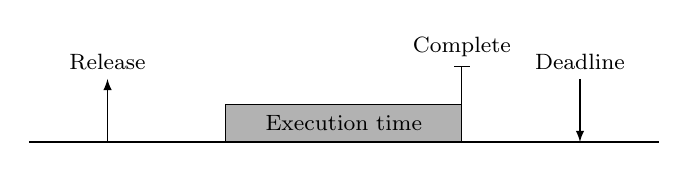
\begin{tikzpicture}[
  yscale = 0.8,
  normal/.style={fill=black!30},
  release/.style={-latex},
  complet/.style={-|},
  every text node part/.style={align=center}
]
%general params
\def\th{.6} %task height
\def\blockdim{(.4,.4)}
\def\arrowdim{(0,.5)}
\def\arrowdimB{(0,.4)}

%axes
\draw[thick, black] (0,0) -- (8, 0);

%L1
\draw[release] (1, 0) -- +(0,1) node[above] {{\footnotesize Release}};
\draw[normal]  (2.5, 0) rectangle +(3, \th) node[midway] {{\footnotesize Execution time}};
\draw[complet] (5.5, 0) -- +(0, 1.2) node[above] {{\footnotesize Complete}};
\draw[release] (7, 1) node[above] {{\footnotesize Deadline}} -- (7,0);

\end{tikzpicture}
}



\newcommand{\mrspSlideBis}{%
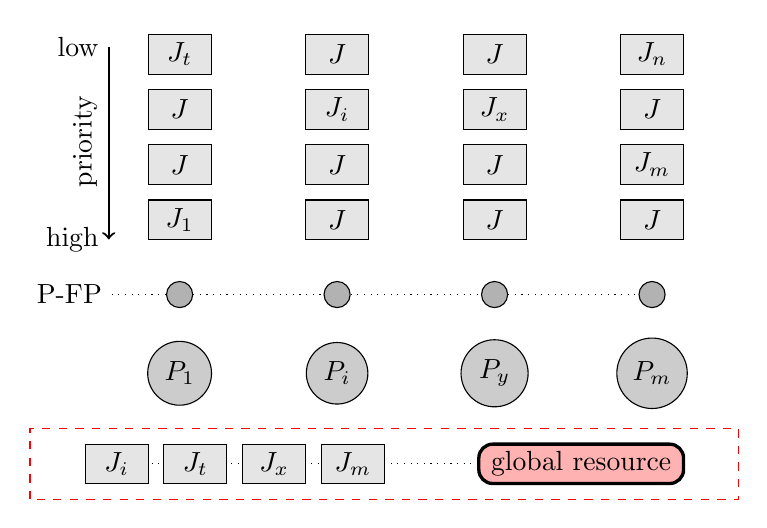
\begin{tikzpicture}[
  every text node part/.style={align=center},
  every circle node/.style={minimum width=.5ex},
  cpusty/.style={fill=gray!40,draw,circle,minimum width=1cm},
  task/.style={fill=black!10},
  sched/.style={fill=black!30,draw,circle,minimum width=1cm},
  ressty/.style={fill=red!30, draw, very thick, rounded corners=5pt}
]
%general params
\def\th{.5} %task height
\def\padding{.7}
\def\offset{.4}

% \partition{1};

  \node[cpusty] (P1) at (0+\offset,-1) {$P_1$};
  \node[sched]  (S1) at (0+\offset,0) {};

  \draw[task] (0.0,\padding*1) rectangle +(0.8, \th) node[midway,black]{$J_1$};
  \draw[task] (0.0,\padding*2) rectangle +(0.8, \th) node[midway,black]{$J$};
  \draw[task] (0.0,\padding*3) rectangle +(0.8, \th) node[midway,black]{$J$};
  \draw[task] (0.0,\padding*4) rectangle +(0.8, \th) node[midway,black]{$J_t$};

  \node[cpusty] (PI) at (2+\offset,-1) {$P_i$};
  \node[sched]  (SI) at (2+\offset,0) {};

  \draw[task] (2,\padding*1) rectangle +(0.8, \th) node[midway,black]{$J$};
  \draw[task] (2,\padding*2) rectangle +(0.8, \th) node[midway,black]{$J$};
  \draw[task] (2,\padding*3) rectangle +(0.8, \th) node[midway,black]{$J_i$};
  \draw[task] (2,\padding*4) rectangle +(0.8, \th) node[midway,black]{$J$};

  \node[cpusty] (PY) at (4.0+\offset,-1) {$P_y$};
  \node[sched]  (SY) at (4.0+\offset,0) {};

  \draw[task] (4,\padding*1) rectangle +(0.8, \th) node[midway,black]{$J$};
  \draw[task] (4,\padding*2) rectangle +(0.8, \th) node[midway,black]{$J$};
  \draw[task] (4,\padding*3) rectangle +(0.8, \th)  node[midway,black]{$J_x$};
  \draw[task] (4,\padding*4) rectangle +(0.8, \th) node[midway,black]{$J$};

  \node[cpusty] (PN) at (6.0+\offset,-1) {$P_m$};
  \node[sched]  (SN) at (6.0+\offset,0) {};

  \draw[task] (6,\padding*1) rectangle +(0.8, \th) node[midway,black]{$J$};
  \draw[task] (6,\padding*2) rectangle +(0.8, \th) node[midway,black]{$J_m$};
  \draw[task] (6,\padding*3) rectangle +(0.8, \th) node[midway,black]{$J$};
  \draw[task] (6,\padding*4) rectangle +(0.8, \th) node[midway,black]{$J_n$};
  
  \draw[dotted] (S1) -- (SI);
  \draw[dotted] (SI) -- (SY);
  \draw[dotted] (SY) -- (SN);

  \node (PFP) at (-1,0) {P-FP};
  \draw[dotted] (PFP) -- (S1);

  \draw[thick,->] (-.5,\padding*4.5) node[left,black]{low} node[rotate=90,left,xshift=-0.5cm,yshift=0.3cm]{priority} -- (-.5,\padding*1) node[left,black]{high};

  \begin{scope} [xshift=-0.8cm, yshift=-2.4cm]

  \draw[dashed, red] (-0.7,-0.2) rectangle (8.3,0.7);

  \draw[dotted] (0,0.25) -- +(5,0);
  \draw[task] (0,0) rectangle +(0.8, \th) node[midway,black]{$J_i$};
  \draw[task] (1,0) rectangle +(0.8, \th) node[midway,black]{$J_t$};
  \draw[task] (2,0) rectangle +(0.8, \th) node[midway,black]{$J_x$};
  \draw[task] (3,0) rectangle +(0.8, \th) node[midway,black]{$J_m$};

  \draw[ressty] (5,0) rectangle +(2.6,.5) node[midway]{global resource};

  % \node[inner sep=0pt] (arrow) at (8.5,1.2) {\includegraphics[width=.1\textwidth]{images/redArrow.png}};

  \end{scope}
 
\end{tikzpicture}
}

% \newcommand{\overheadsSuffered}[2]{%
% \begin{tikzpicture}[
%   xscale=#1,
%   yscale=#2,
%   every node/.append style={transform shape},
%   queuesty/.style={fill=white, very thick, font=\tiny},
%   srpsty/.style={fill=white, draw, circle, text width=.17cm, font=\tiny, very thick},
%   numsty/.style={text width=.1cm, font=\tiny},
%   arrow/.style={->},
%   littletext/.style={font=\sffamily\tiny,inner sep=0pt,outer sep=-2pt,fill=white},
%   ressty/.style={fill=red!30, draw, very thick, rounded corners=5pt},
%   emptytask/.style={rectangle, minimum width=.7cm,font=\footnotesize},
%   taskHolder/.style={fill=blue!90, draw, rectangle, minimum width=.7cm,font=\footnotesize},
%   taskWaiting/.style={fill=blue!70, draw, rectangle, minimum width=.7cm,font=\footnotesize,postaction={pattern=north east lines, very thin, pattern color=white}},
%   taskAccess/.style={fill=blue!30, draw, rectangle, minimum width=.7cm,font=\footnotesize},
%   taskNotAccess/.style={fill=white, draw, rectangle, minimum width=.7cm,font=\footnotesize}]

% \def\blockdim{(.7,.25)}

% \draw[arrow] (2.2,5.25) to[out=90,in=0] (2.35,6.6);

% \begin{scope}[xshift=2.2cm, yshift=5cm]
%   \coordinate (SRPnode) at (0,0);

%   \draw[dashed,purple] (-1.5,-0.78) -- (0.27,-0.78);

%   \node[taskNotAccess]  (T1)  at (-0.8,-0.50)  {};
%   \node[emptytask]      (TP1) at (-0.8,-0.75) {$\cdots$};
%   \node[taskWaiting]     (T2)  at (-0.8,-1.00)  {};
%   \node[emptytask]      (TP1) at (-0.8,-1.25) {$\cdots$};
%   \node[taskAccess]     (T3)  at (-0.8,-1.50)  {};
%   \node[emptytask]      (TP1) at (-0.8,-1.75) {$\cdots$};
%   \node[taskNotAccess]  (T4)  at (-0.8,-2.00)  {};
%   \node[emptytask]      (TP1) at (-0.8,-2.25) {$\cdots$};
%   \node[taskNotAccess]     (T5)  at (-0.8,-2.50)  {};

%   \draw[dashed, thin] ([shift={(-1.5,0)}]SRPnode) node[right,xshift=.1cm,littletext]{Partition$_2$} rectangle ([shift={(.3,-.15)}]T5.south-|SRPnode.east);

%   \node[srpsty] (SRP) at (SRPnode) {}; \node[font=\sffamily\tiny] at(SRPnode.west){SRP};
%   \draw[arrow] (T2.east) to[out=0,in=270] (SRP.south);

%   \draw[red] ([shift={(-.4,.17)}]T2) rectangle ([shift={(.25,-.05)}]T5.south-|T5.east);

%   \draw[arrow,red] (-0.35,-3.05) -- ([shift={(.1,-.05)}]T5.south-|T3.east);

% \end{scope}

\section{Introduction}

	\begin{frame}
	\frametitle{Real-Time System Model}
	\framesubtitle{Platform}	

		\begin{figure}
			\centering
			\scalebox{.8}{\mrspSlide}
			\caption{Partitioned Fixed-Priority scheduler on a platform with $m$ processors ($P_1$, \dots, $P_m$) and a global resource}
		\end{figure}

	\end{frame}
\newcommand{\waitingtime}{
\begin{tikzpicture}[
  yscale = 0.8,
  normal/.style={ fill=black!30},
  resource/.style={ fill=black!80},
  waiting/.style={fill=white},
  busywait/.style={fill=black!10, postaction={pattern=north east lines, very thin}},
  release/.style={-latex},
  request/.style={-o},
  complet/.style={-|},
  important/.style={color=red,thick,|-|},
  every text node part/.style={align=center}
]
%general params
\def\th{.4} %task height
\def\tyDown{0} %task a asse y
\def\tyUp{1}
\def\blockdim{(.4,.4)}
\def\arrowdim{(0,.5)}
\def\arrowdimB{(0,.4)}
\coordinate (legend) at (-0.5,2.3);

\begin{scope}

\path(-1.4, 2)node[below]{\textcolor{red}{(1)}};
\path(3.7, 2)node[below] {\textcolor{red}{(2)}};

%tasklines
\draw[very thin, gray] (-.7,\tyDown)node[above,left,black]{$P_2$} -- +(3.2,0);
\draw[very thin, gray] (-.7,\tyUp)node[above,left,black]{$P_1$} -- +(3.2,0);

%axes
\draw[thick, black, -] (-.5,-0.7) -- (-.5, 1.8);
\draw[thick, black, ->] (-1,-.5) -- (2.7, -.5);
% \foreach \x in {0,...,2}\draw[thin, black] (\x, -.6) -- (\x, -.4);

%Processor 1 ==> \tyUp

\draw[release] (0,\tyUp) -- +(0,.8);
\draw[normal]   (0, \tyUp) rectangle +(0.4, \th) node[midway] {{\footnotesize $J_1$}};
\draw[request] (0.4,\tyUp) -- +(0,.8);
\draw[resource] (0.4, \tyUp) rectangle +(0.5, \th) node[color=white,midway] {{\footnotesize  $J_1$}};
\draw[release] (0.9,\tyUp) -- +(0,.8)node[above] {{\tiny $J_3$}};
\draw[normal]   (0.9, \tyUp) rectangle +(0.6, \th) node[midway] {{\footnotesize $J_3$}};
\draw[complet] (1.5,\tyUp) -- +(0, .7);
\draw[resource] (1.5, \tyUp) rectangle +(0.4, \th) node[color=white,midway] {{\footnotesize  $J_1$}};
\draw[complet] (1.9,\tyUp) -- +(0, .7);

%Processor 2 ==> \tyDown

\draw[release] (0.2,\tyDown) -- +(0,.8);
\draw[normal]   (0.2, \tyDown) rectangle +(0.6, \th) node[midway] {{\footnotesize $J_2$}};
\draw[request] (0.8,\tyDown) -- +(0,.8);

\path(0.8, -.6)node[below]{{\tiny $t_1$}};
\draw[thin, black] (0.8, -.6) -- (0.8, -.4);

\path(1.9, -.6)node[below]{{\tiny $t_2$}};
\draw[thin, black] (1.9, -.6) -- (1.9, -.4);

\draw[important] (0.82,\tyDown + 0.25) -- +(1.06,0) node[midway,yshift=0.2cm]{\scriptsize \textcolor{blue}{(a)}};

\draw[resource] (1.9, \tyDown) rectangle +(0.6, \th) node[color=white,midway] {{\footnotesize  $J_2$}};
\draw[complet] (2.5,\tyDown) -- +(0, .7);

\path(0, -1)node[xshift=1cm,below]{{\footnotesize \textcolor{blue}{(a)} queueing time}};

\end{scope}

\begin{scope}[xshift=4.8cm]

%tasklines
\draw[very thin, gray] (-.7,\tyDown) -- +(3.2,0);
\draw[very thin, gray] (-.7,\tyUp) -- +(3.2,0);

%axes
\draw[thick, black, -] (-.5,-0.7) -- (-.5, 1.8);
\draw[thick, black, ->] (-1,-.5) -- (2.7, -.5) node[below] {{\footnotesize time}};
% \foreach \x in {0,...,2}\draw[thin, black] (\x, -.6) -- (\x, -.4);

%Processor 1 ==> \tyUp

\draw[release] (0,\tyUp) -- +(0,.8);
\draw[normal]   (0, \tyUp) rectangle +(0.4, \th) node[midway] {{\footnotesize $J_1$}};
\draw[request] (0.4,\tyUp) -- +(0,.8);

\draw[release] (0.9,\tyUp) -- +(0,.8)node[above] {{\tiny $J_3$}};

\draw[resource] (0.4, \tyUp) rectangle +(1.5, \th) node[color=white,midway] {{\footnotesize  $J_1$}};

\draw [decorate,decoration={brace,amplitude=3pt,mirror,raise=2pt},yshift=0pt,red]
(0.92,\tyUp - 0.05) -- +(1.88 - 0.92,0) node[midway, yshift=-0.37cm]{\scriptsize \textcolor{blue}{(b)}};

\draw[complet] (1.9,\tyUp) -- +(0, .7);

\draw[normal]   (1.9, \tyUp) rectangle +(0.6, \th) node[midway] {{\footnotesize $J_3$}};
\draw[complet] (2.5,\tyUp) -- +(0, .7);

%Processor 2 ==> \tyDown

\draw[release] (0.2,\tyDown) -- +(0,.8);
\draw[normal]   (0.2, \tyDown) rectangle +(0.5, \th) node[midway] {{\footnotesize $J_2$}};
\draw[request] (0.7,\tyDown) -- +(0,.8);

\path(0.7, -.6)node[below]{{\tiny $t_1$}};
\draw[thin, black] (0.7, -.6) -- (0.7, -.4);

\path(1.9, -.6)node[below]{{\tiny $t_2$}};
\draw[thin, black] (1.9, -.6) -- (1.9, -.4);

\draw[resource] (1.9, \tyDown) rectangle +(0.5, \th) node[color=white,midway] {{\footnotesize  $J_2$}};
\draw[complet] (2.4,\tyDown) -- +(0, .7);

\path(0, -1)node[xshift=1cm,below]{{\footnotesize \textcolor{blue}{(b)} "independence preserving"}};

\end{scope}

\draw[normal]   ($(   0,0.5) + (legend)$) node[below, xshift=0.2cm]{\tiny executing} rectangle +\blockdim;
\draw[resource] ($(1.75,0.5) + (legend)$) node[below, xshift=0.2cm]{\tiny resource} rectangle +\blockdim;
\draw[release]  ($( 3.5,0.5) + (legend)$) node[below]{\tiny job release}      -- +\arrowdim;
\draw[request]  ($(5.25,0.5) + (legend)$) node[below]{\tiny request}     -- +\arrowdim;
\draw[complet]  ($(   7,0.5) + (legend)$) node[below]{\tiny completion}   -- +\arrowdimB;

\end{tikzpicture}
}

%%%%%%%%%%%%%%%%%%%%%%%%%%%%%%%%%%%%%%%%%%%%%%%%%%%%%%%%%%%%%%%%%%%%%%%%%%%%%%%%%%%%%%%%%%%%%%%%%%%%

\newcommand{\migrationSolution}{
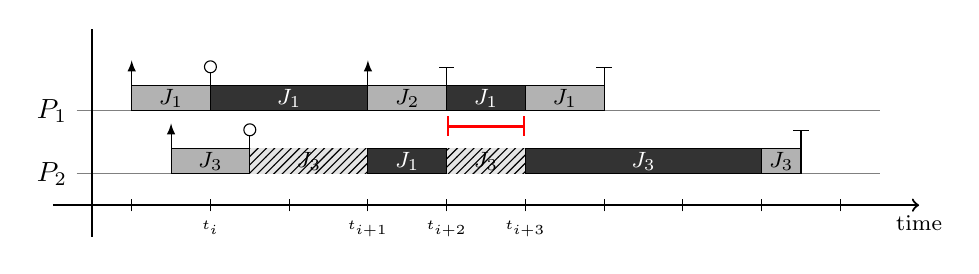
\begin{tikzpicture}[
  yscale = 0.8,
  normal/.style={ fill=black!30},
  resource/.style={ fill=black!80},
  waiting/.style={fill=white},
  busywait/.style={fill=black!10, postaction={pattern=north east lines, very thin}},
  release/.style={-latex},
  request/.style={-o},
  complet/.style={-|},
  important/.style={color=red,thick,|-|},
  every text node part/.style={align=center}
]
%general params
\def\th{.4} %task height
\def\offeset{.25} %task height
\def\tyDown{0} %task a asse y
\def\tyUp{1}
\def\blockdim{(.4,.4)}
\def\arrowdim{(0,.5)}
\def\arrowdimB{(0,.4)}
\coordinate (legend) at (0.5,2.5);

%tasklines
\draw[very thin, gray] (-.7,\tyDown)node[above,left,black]{$P_2$} -- +(10.2,0);
\draw[very thin, gray] (-.7,\tyUp)node[above,left,black]{$P_1$} -- +(10.2,0);

%axes
\draw[thick, black, -] (-.5,-1) -- (-.5, 2.3);
\draw[thick, black, ->] (-1,-.5) -- (10, -.5) node[below] {{\footnotesize time}};
\foreach \x in {0,...,9}\draw[thin, black] (\x, -.6) -- (\x, -.4);

%Processor 1 ==> \tyUp

\draw[normal]   (0, \tyUp) rectangle +(1, \th) node[midway] {{\footnotesize $J_1$}};
\draw[resource] (1, \tyUp) rectangle +(2, \th) node[color=white,midway] {{\footnotesize  $J_1$}};
\draw[normal]   (3, \tyUp) rectangle +(1, \th) node[midway] {{\footnotesize $J_2$}};
\draw[resource] (4, \tyUp) rectangle +(1, \th) node[color=white,midway] {{\footnotesize  $J_1$}};
\draw[normal]   (5, \tyUp) rectangle +(1, \th) node[midway] {{\footnotesize $J_1$}};

\draw[release] (0,\tyUp) -- +(0,.8);
\draw[request] (1,\tyUp) -- +(0,.8);
\path(1, -.6)node[below]{{\tiny $t_{i}$}};
\draw[release] (3,\tyUp) -- +(0,.8);
\path(3, -.6)node[below]{{\tiny $t_{i+1}$}};
\draw[complet] (4,\tyUp) -- +(0, .7);
\path(4, -.6)node[below]{{\tiny $t_{i+2}$}};
\draw[complet] (6,\tyUp) -- +(0, .7);

%Processor 2 ==> \tyDown

\draw[normal]   (0.5, \tyDown) rectangle +(1, \th) node[midway] {{\footnotesize $J_3$}};
\fill[busywait] (1.5, \tyDown) rectangle +(1.5, \th) node[midway] {{\footnotesize $J_3$}};
\draw[resource] (3, \tyDown) rectangle +(1, \th) node[color=white,midway] {{\footnotesize  $J_1$}};
\fill[busywait] (4, \tyDown) rectangle +(1, \th) node[midway] {{\footnotesize $J_3$}};
\draw[resource] (5, \tyDown) rectangle +(3, \th) node[color=white,midway] {{\footnotesize  $J_3$}};
\draw[normal]   (8, \tyDown) rectangle +(0.5, \th) node[midway] {{\footnotesize $J_3$}};

\draw[release] (0.5,\tyDown) -- +(0,.8);
\draw[request] (1.5,\tyDown) -- +(0,.8);
\path(5, -.6)node[below]{{\tiny $t_{i+3}$}};
\draw[complet] (8.5,\tyDown) -- +(0, .7);

\draw[important] (4,\tyUp - \offeset) -- (5,\tyUp - \offeset);

\end{tikzpicture}
}

\newcommand{\agentSolution}{
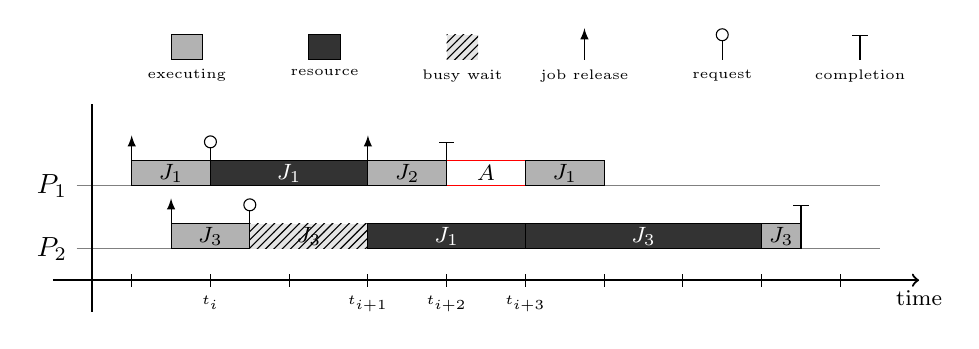
\begin{tikzpicture}[
  yscale = 0.8,
  normal/.style={ fill=black!30},
  resource/.style={ fill=black!80},
  waiting/.style={fill=white,draw=red},
  busywait/.style={fill=black!10, postaction={pattern=north east lines, very thin}},
  release/.style={-latex},
  request/.style={-o},
  complet/.style={-|},
  important/.style={color=red,thick,|-|},
  every text node part/.style={align=center}
]
%general params
\def\th{.4} %task height
\def\tyDown{0} %task a asse y
\def\tyUp{1}
\def\blockdim{(.4,.4)}
\def\arrowdim{(0,.5)}
\def\arrowdimB{(0,.4)}
\coordinate (legend) at (0.5,2.5);

%tasklines
\draw[very thin, gray] (-.7,\tyDown)node[above,left,black]{$P_2$} -- +(10.2,0);
\draw[very thin, gray] (-.7,\tyUp)node[above,left,black]{$P_1$} -- +(10.2,0);

%axes
\draw[thick, black, -] (-.5,-1) -- (-.5, 2.3);
\draw[thick, black, ->] (-1,-.5) -- (10, -.5) node[below] {{\footnotesize time}};
\foreach \x in {0,...,9}\draw[thin, black] (\x, -.6) -- (\x, -.4);

%Processor 1 ==> \tyUp

\draw[normal]   (0, \tyUp) rectangle +(1, \th) node[midway] {{\footnotesize $J_1$}};
\draw[resource] (1, \tyUp) rectangle +(2, \th) node[color=white,midway] {{\footnotesize  $J_1$}};
\draw[normal]   (3, \tyUp) rectangle +(1, \th) node[midway] {{\footnotesize $J_2$}};
\draw[waiting]   (4, \tyUp) rectangle +(1, \th) node[midway] {{\footnotesize $A$}};
\draw[normal]   (5, \tyUp) rectangle +(1, \th) node[midway] {{\footnotesize $J_1$}};

\draw[release] (0,\tyUp) -- +(0,.8);
\draw[request] (1,\tyUp) -- +(0,.8);
\path(1, -.6)node[below]{{\tiny $t_{i}$}};
\draw[release] (3,\tyUp) -- +(0,.8);
\path(3, -.6)node[below]{{\tiny $t_{i+1}$}};
\draw[complet] (4,\tyUp) -- +(0, .7);
\path(4, -.6)node[below]{{\tiny $t_{i+2}$}};

%Processor 2 ==> \tyDown

\draw[normal]   (0.5, \tyDown) rectangle +(1, \th) node[midway] {{\footnotesize $J_3$}};
\fill[busywait] (1.5, \tyDown) rectangle +(1.5, \th) node[midway] {{\footnotesize $J_3$}};
\draw[resource] (3, \tyDown) rectangle +(2, \th) node[color=white,midway] {{\footnotesize  $J_1$}};
\draw[resource] (5, \tyDown) rectangle +(3, \th) node[color=white,midway] {{\footnotesize  $J_3$}};
\draw[normal]   (8, \tyDown) rectangle +(0.5, \th) node[midway] {{\footnotesize $J_3$}};

\draw[release] (0.5,\tyDown) -- +(0,.8);
\draw[request] (1.5,\tyDown) -- +(0,.8);
\path(5, -.6)node[below]{{\tiny $t_{i+3}$}};
\draw[complet] (8.5,\tyDown) -- +(0, .7);

\draw[normal]   ($(   0,0.5) + (legend)$) node[below, xshift=0.2cm]{\tiny executing} rectangle +\blockdim;
\draw[resource] ($(1.75,0.5) + (legend)$) node[below, xshift=0.2cm]{\tiny resource} rectangle +\blockdim;
\fill[busywait] ($( 3.5,0.5) + (legend)$) node[below, xshift=0.2cm]{\tiny busy wait} rectangle +\blockdim;
\draw[release]  ($(5.25,0.5) + (legend)$) node[below]{\tiny job release}      -- +\arrowdim;
\draw[request]  ($(   7,0.5) + (legend)$) node[below]{\tiny request}     -- +\arrowdim;
\draw[complet]  ($(8.75,0.5) + (legend)$) node[below]{\tiny completion}   -- +\arrowdimB;

\end{tikzpicture}
}
\newcommand{\MrsPProtocols}{%
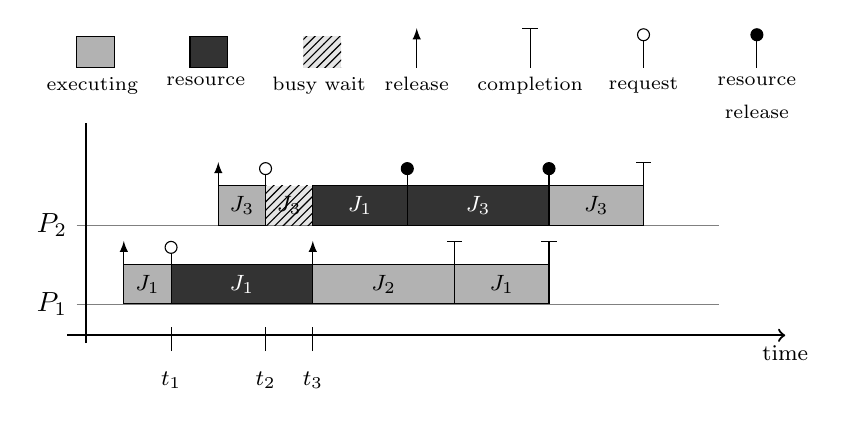
\begin{tikzpicture}[
  xscale=1.2,
  normal/.style={fill=black!30},
  release/.style={-latex},
  complet/.style={-|},
  every text node part/.style={align=center},
  important/.style={color=red,thick,-,dashed},
  resource/.style={ fill=black!80},
  waiting/.style={fill=white},
  busywait/.style={fill=black!10,postaction={pattern=north east lines, very thin}},
  request/.style={-o},
  unlock/.style={-*},
]
%general params
\def\th{.5} %task height
\def\blockdim{(.4,.4)}
\def\arrowdim{(0,.5)}
\def\arrowdimB{(0,.4)}

\def\tyTwo{1}
\def\tyOne{0}
%axes

%tasklines
\def\tasklinelength{(6.8,0)}
\draw[very thin, gray] (-.5,\tyOne)node[above,left,black]{$P_1$} -- +\tasklinelength;
\draw[very thin, gray] (-.5,\tyTwo)node[above,left,black]{$P_2$} -- +\tasklinelength;

%axes
\draw[thick, black, -] (-.4,-.5) -- (-.4, 2.3);
\draw[thick, black, ->] (-.6,-.4) -- (7, -.4) node[below] {{\footnotesize time}};
% \foreach \x in {0,...,5} \draw[thin, black] (\x, -.6) -- (\x, -.3);

\draw[release]  (0.0, \tyOne) -- +(0,.8);
\draw[normal]   (0.0, \tyOne) rectangle +(0.5, \th) node[midway] {{\footnotesize $J_1$}};
\draw[request]  (0.5, \tyOne) -- +(0,.8);
\path(0.5, -1.2) node[above]{{\footnotesize $t_1$}};
\draw[thin, black] (0.5, -.6) -- (0.5, -.3);
\draw[resource] (0.5, \tyOne) rectangle +(1.5, \th)   node[color=white,midway] {{\footnotesize  $J_1$}};

\draw[thin, black] (2.0, -.6) -- (2.0, -.3);
\path(2.0, -1.2) node[above]{{\footnotesize $t_3$}};
\draw[release]  (2.0, \tyOne) -- +(0,.8);
\draw[normal]   (2.0, \tyOne) rectangle +(1.5, \th) node[midway] {{\footnotesize $J_2$}};
\draw[complet]  (3.5, \tyOne) -- +(0,.8);

\draw[normal]   (3.5, \tyOne) rectangle +(1.0, \th) node[midway] {{\footnotesize $J_1$}};
\draw[complet]  (4.5, \tyOne) -- +(0,.8);


\draw[release]  (1.0, \tyTwo) -- +(0,.8);
\draw[normal]   (1.0, \tyTwo) rectangle +(0.5, \th) node[midway] {{\footnotesize $J_3$}};
\draw[request]  (1.5, \tyTwo) -- +(0,.8);
\path(1.5, -1.2) node[above]{{\footnotesize $t_2$}};
\draw[thin, black] (1.5, -.6) -- (1.5, -.3);
\fill[busywait] (1.5, \tyTwo) rectangle +(0.5, \th)   node[midway] {{\footnotesize $J_3$}};

\draw[resource] (2.0, \tyTwo) rectangle +(1.0, \th)   node[color=white,midway] {{\footnotesize  $J_1$}};
\draw[unlock]   (3.0, \tyTwo) -- +(0,.8);

\draw[resource] (3.0, \tyTwo) rectangle +(1.5, \th)   node[color=white,midway] {{\footnotesize  $J_3$}};
\draw[unlock]   (4.5, \tyTwo) -- +(0,.8);

\draw[normal]   (4.5, \tyTwo) rectangle +(1.0, \th) node[midway] {{\footnotesize $J_3$}};
\draw[complet]  (5.5, \tyTwo) -- +(0,.8);


\coordinate (legend) at (0,2.5);

\draw[normal]   ($(-0.5,0.5) + (legend)$) node[below, xshift=0.2cm]{\scriptsize executing} rectangle +\blockdim;
\draw[resource] ($(0.7,0.5) + (legend)$) node[below, xshift=0.2cm]{\scriptsize resource} rectangle +\blockdim;
\fill[busywait] ($(1.9,0.5) + (legend)$) node[below, xshift=0.2cm]{\scriptsize busy wait} rectangle +\blockdim;
\draw[release]  ($(3.1,0.5) + (legend)$) node[below]{\scriptsize release}      -- +\arrowdim;
\draw[complet]  ($(4.3,0.5) + (legend)$) node[below]{\scriptsize completion}   -- +\arrowdim;
\draw[request]  ($(5.5,0.5) + (legend)$) node[below]{\scriptsize request}     -- +\arrowdim;
\draw[unlock]   ($(6.7,0.5) + (legend)$) node[below]{\scriptsize resource \\ \scriptsize release}     -- +\arrowdim;

\end{tikzpicture}
}




\newcommand{\MrsPProtocolsHarder}{%
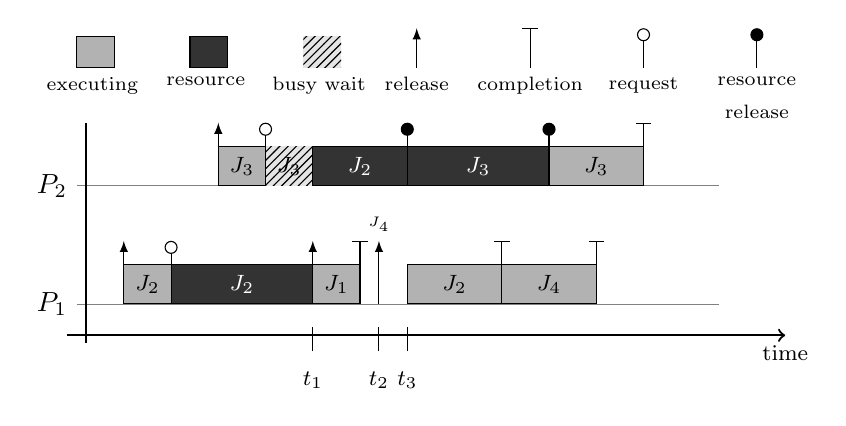
\begin{tikzpicture}[
  xscale=1.2,
  normal/.style={fill=black!30},
  release/.style={-latex},
  complet/.style={-|},
  every text node part/.style={align=center},
  important/.style={color=red,thick,-,dashed},
  resource/.style={ fill=black!80},
  waiting/.style={fill=white},
  busywait/.style={fill=black!10,postaction={pattern=north east lines, very thin}},
  request/.style={-o},
  unlock/.style={-*},
]
%general params
\def\th{.5} %task height
\def\blockdim{(.4,.4)}
\def\arrowdim{(0,.5)}
\def\arrowdimB{(0,.4)}

\def\tyTwo{1.5}
\def\tyOne{0}
%axes

%tasklines
\def\tasklinelength{(6.8,0)}
\draw[very thin, gray] (-.5,\tyOne)node[above,left,black]{$P_1$} -- +\tasklinelength;
\draw[very thin, gray] (-.5,\tyTwo)node[above,left,black]{$P_2$} -- +\tasklinelength;

%axes
\draw[thick, black, -] (-.4,-.5) -- (-.4, 2.3);
\draw[thick, black, ->] (-.6,-.4) -- (7, -.4) node[below] {{\footnotesize time}};
% \foreach \x in {0,...,5} \draw[thin, black] (\x, -.6) -- (\x, -.3);

\draw[release]  (0.0, \tyOne) -- +(0,.8);
\draw[normal]   (0.0, \tyOne) rectangle +(0.5, \th) node[midway] {{\footnotesize $J_2$}};
\draw[request]  (0.5, \tyOne) -- +(0,.8);
% \path(0.5, -1.2) node[above]{{\footnotesize $t_1$}};
\draw[resource] (0.5, \tyOne) rectangle +(1.5, \th)   node[color=white,midway] {{\footnotesize  $J_2$}};

\draw[thin, black] (2.0, -.6) -- (2.0, -.3);
\path(2.0, -1.2) node[above]{{\footnotesize $t_1$}};
\draw[release]  (2.0, \tyOne) -- +(0,.8);
\draw[normal]   (2.0, \tyOne) rectangle +(0.5, \th) node[midway] {{\footnotesize $J_1$}};
\draw[complet]  (2.5, \tyOne) -- +(0,.8);

\draw[release]  (2.7, \tyOne) -- +(0,.8) node[above] {{\tiny $J_4$}};

\draw[thin, black] (2.7, -.6) -- (2.7, -.3);
\path(2.7, -1.2) node[above]{{\footnotesize $t_2$}};

\draw[thin, black] (3.0, -.6) -- (3.0, -.3);
\path(3.0, -1.2) node[above]{{\footnotesize $t_3$}};

\draw[normal]   (3.0, \tyOne) rectangle +(1.0, \th) node[midway] {{\footnotesize $J_2$}};
\draw[complet]  (4.0, \tyOne) -- +(0,.8);

\draw[normal]   (4.0, \tyOne) rectangle +(1.0, \th) node[midway] {{\footnotesize $J_4$}};
\draw[complet]  (5.0, \tyOne) -- +(0,.8);

\draw[release]  (1.0, \tyTwo) -- +(0,.8);
\draw[normal]   (1.0, \tyTwo) rectangle +(0.5, \th) node[midway] {{\footnotesize $J_3$}};
\draw[request]  (1.5, \tyTwo) -- +(0,.8);

% \draw[thin, black] (1.5, -.6) -- (1.5, -.3);
\fill[busywait] (1.5, \tyTwo) rectangle +(0.5, \th)   node[midway] {{\footnotesize $J_3$}};

\draw[resource] (2.0, \tyTwo) rectangle +(1.0, \th)   node[color=white,midway] {{\footnotesize  $J_2$}};
\draw[unlock]   (3.0, \tyTwo) -- +(0,.8);

\draw[resource] (3.0, \tyTwo) rectangle +(1.5, \th)   node[color=white,midway] {{\footnotesize  $J_3$}};
\draw[unlock]   (4.5, \tyTwo) -- +(0,.8);

\draw[normal]   (4.5, \tyTwo) rectangle +(1.0, \th) node[midway] {{\footnotesize $J_3$}};
\draw[complet]  (5.5, \tyTwo) -- +(0,.8);


\coordinate (legend) at (0,2.5);

\draw[normal]   ($(-0.5,0.5) + (legend)$) node[below, xshift=0.2cm]{\scriptsize executing} rectangle +\blockdim;
\draw[resource] ($(0.7,0.5) + (legend)$) node[below, xshift=0.2cm]{\scriptsize resource} rectangle +\blockdim;
\fill[busywait] ($(1.9,0.5) + (legend)$) node[below, xshift=0.2cm]{\scriptsize busy wait} rectangle +\blockdim;
\draw[release]  ($(3.1,0.5) + (legend)$) node[below]{\scriptsize release}      -- +\arrowdim;
\draw[complet]  ($(4.3,0.5) + (legend)$) node[below]{\scriptsize completion}   -- +\arrowdim;
\draw[request]  ($(5.5,0.5) + (legend)$) node[below]{\scriptsize request}     -- +\arrowdim;
\draw[unlock]   ($(6.7,0.5) + (legend)$) node[below]{\scriptsize resource \\ \scriptsize release}     -- +\arrowdim;

\end{tikzpicture}
}


\newcommand{\MrsPProtocolsHarderBis}{%
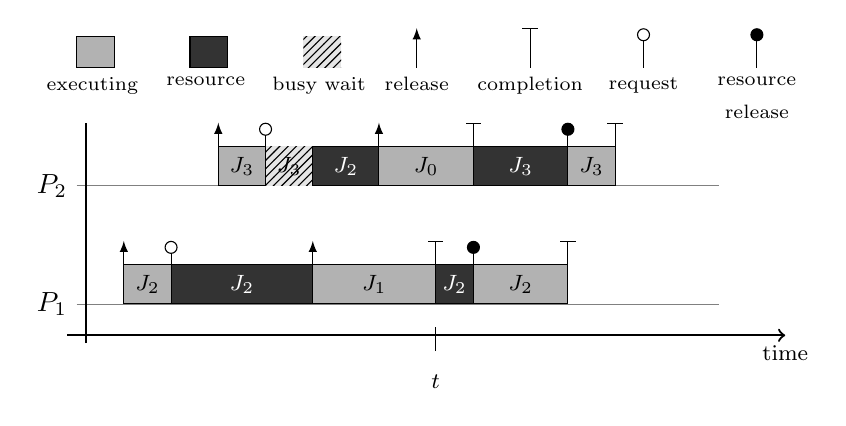
\begin{tikzpicture}[
  xscale=1.2,
  normal/.style={fill=black!30},
  release/.style={-latex},
  complet/.style={-|},
  every text node part/.style={align=center},
  important/.style={color=red,thick,-,dashed},
  resource/.style={ fill=black!80},
  waiting/.style={fill=white},
  busywait/.style={fill=black!10,postaction={pattern=north east lines, very thin}},
  request/.style={-o},
  unlock/.style={-*},
]
%general params
\def\th{.5} %task height
\def\blockdim{(.4,.4)}
\def\arrowdim{(0,.5)}
\def\arrowdimB{(0,.4)}

\def\tyTwo{1.5}
\def\tyOne{0}
%axes

%tasklines
\def\tasklinelength{(6.8,0)}
\draw[very thin, gray] (-.5,\tyOne)node[above,left,black]{$P_1$} -- +\tasklinelength;
\draw[very thin, gray] (-.5,\tyTwo)node[above,left,black]{$P_2$} -- +\tasklinelength;

%axes
\draw[thick, black, -] (-.4,-.5) -- (-.4, 2.3);
\draw[thick, black, ->] (-.6,-.4) -- (7, -.4) node[below] {{\footnotesize time}};
% \foreach \x in {0,...,5} \draw[thin, black] (\x, -.6) -- (\x, -.3);

\draw[release]  (0.0, \tyOne) -- +(0,.8);
\draw[normal]   (0.0, \tyOne) rectangle +(0.5, \th) node[midway] {{\footnotesize $J_2$}};
\draw[request]  (0.5, \tyOne) -- +(0,.8);

\draw[resource] (0.5, \tyOne) rectangle +(1.5, \th)   node[color=white,midway] {{\footnotesize  $J_2$}};

\draw[release]  (2.0, \tyOne) -- +(0,.8);
\draw[normal]   (2.0, \tyOne) rectangle +(1.3, \th) node[midway] {{\footnotesize $J_1$}};
\draw[complet]  (3.3, \tyOne) -- +(0,.8);

\draw[resource] (3.3, \tyOne) rectangle +(0.4, \th)   node[color=white,midway] {{\footnotesize  $J_2$}};
\draw[unlock]   (3.7, \tyOne) -- +(0,.8);

\draw[normal]   (3.7, \tyOne) rectangle +(1.0, \th) node[midway] {{\footnotesize $J_2$}};
\draw[complet]  (4.7, \tyOne) -- +(0,.8);


\draw[release]  (1.0, \tyTwo) -- +(0,.8);
\draw[normal]   (1.0, \tyTwo) rectangle +(0.5, \th) node[midway] {{\footnotesize $J_3$}};
\draw[request]  (1.5, \tyTwo) -- +(0,.8);

\fill[busywait] (1.5, \tyTwo) rectangle +(0.5, \th)   node[midway] {{\footnotesize $J_3$}};

\draw[resource] (2.0, \tyTwo) rectangle +(0.7, \th)   node[color=white,midway] {{\footnotesize  $J_2$}};
% \draw[unlock]   (3.0, \tyTwo) -- +(0,.8);

\draw[release]  (2.7, \tyTwo) -- +(0,.8);
\draw[normal]   (2.7, \tyTwo) rectangle +(1, \th) node[midway] {{\footnotesize $J_0$}};
\draw[complet]  (3.7, \tyTwo) -- +(0,.8);

\draw[thin, black] (3.3, -.6) -- (3.3, -.3);
\path(3.3, -1.2) node[above]{{\footnotesize $t$}};

\draw[resource] (3.7, \tyTwo) rectangle +(1.0, \th)   node[color=white,midway] {{\footnotesize  $J_3$}};
\draw[unlock]   (4.7, \tyTwo) -- +(0,.8);

\draw[normal]   (4.7, \tyTwo) rectangle +(0.5, \th) node[midway] {{\footnotesize $J_3$}};
\draw[complet]  (5.2, \tyTwo) -- +(0,.8);


\coordinate (legend) at (0,2.5);

\draw[normal]   ($(-0.5,0.5) + (legend)$) node[below, xshift=0.2cm]{\scriptsize executing} rectangle +\blockdim;
\draw[resource] ($(0.7,0.5) + (legend)$) node[below, xshift=0.2cm]{\scriptsize resource} rectangle +\blockdim;
\fill[busywait] ($(1.9,0.5) + (legend)$) node[below, xshift=0.2cm]{\scriptsize busy wait} rectangle +\blockdim;
\draw[release]  ($(3.1,0.5) + (legend)$) node[below]{\scriptsize release}      -- +\arrowdim;
\draw[complet]  ($(4.3,0.5) + (legend)$) node[below]{\scriptsize completion}   -- +\arrowdim;
\draw[request]  ($(5.5,0.5) + (legend)$) node[below]{\scriptsize request}     -- +\arrowdim;
\draw[unlock]   ($(6.7,0.5) + (legend)$) node[below]{\scriptsize resource \\ \scriptsize release}     -- +\arrowdim;

\end{tikzpicture}
}
\newcommand{\SuspOrSpin}{
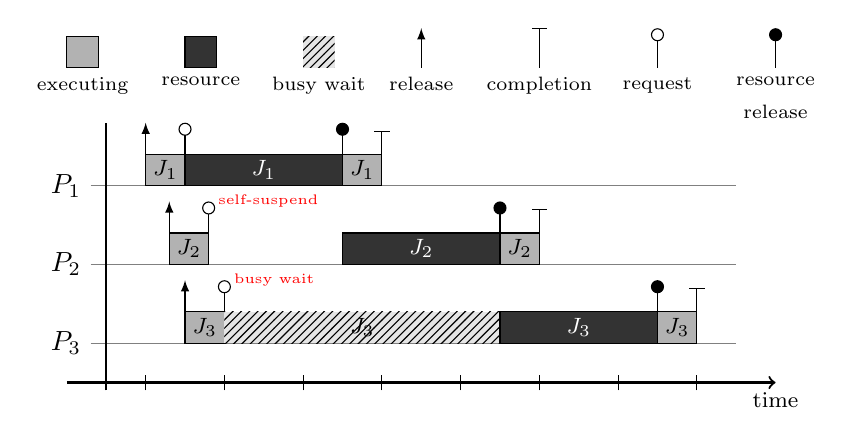
\begin{tikzpicture}[
  normal/.style={ fill=black!30},
  resource/.style={ fill=black!80},
  waiting/.style={fill=white},
  busywait/.style={fill=black!10, postaction={pattern=north east lines, very thin}},
  release/.style={-latex},
  request/.style={-o},
  complet/.style={-|},
  important/.style={color=red,thick,|-|},
  every text node part/.style={align=center},
  unlock/.style={-*}
]
%general params
\def\th{.4} %task height
\def\offeset{.25} %task height
\def\tyDown{0} %task a asse y
\def\tyUp{1}
\def\tyAbove{2}
\def\blockdim{(.4,.4)}
\def\arrowdim{(0,.5)}
\def\arrowdimB{(0,.4)}
\coordinate (legend) at (0.5,2.5);

%tasklines
\draw[very thin, gray] (-.7,\tyDown)node[above,left,black]{$P_3$} --    +(8.2,0);
\draw[very thin, gray] (-.7,\tyUp)node[above,left,black]  {$P_2$} --    +(8.2,0);
\draw[very thin, gray] (-.7,\tyAbove)node[above,left,black]  {$P_1$} -- +(8.2,0);

%axes
\draw[thick, black, -] (-.5,-0.6) -- (-.5, 2.8);
\draw[thick, black, ->] (-1,-.5) -- (8, -.5) node[below] {{\footnotesize time}};
\foreach \x in {0,...,7}\draw[thin, black] (\x, -.6) -- (\x, -.4);

%Processor 1 ==> \tyAbove

\draw[release] (0,    \tyAbove) -- +(0,.8);
\draw[normal]   (0,   \tyAbove) rectangle +(0.5, \th) node[midway] {{\footnotesize $J_1$}};
\draw[request] (0.5,  \tyAbove) -- +(0,.8);
\draw[resource] (0.5, \tyAbove) rectangle +(2, \th) node[color=white,midway] {{\footnotesize  $J_1$}};
\draw[unlock]   (2.5, \tyAbove) -- +(0,.8);
\draw[normal]   (2.5, \tyAbove) rectangle +(0.5, \th) node[midway] {{\footnotesize $J_1$}};
\draw[complet] (3,    \tyAbove) -- +(0, .7);


%Processor 2 ==> \tyUp

\def\offsetA{.3}
\def\offsetB{2}

\draw[release]  (0.0+\offsetA, \tyUp) -- +(0,.8);
\draw[normal]   (0.0+\offsetA, \tyUp) rectangle +(0.5, \th) node[midway] {{\footnotesize $J_2$}};
\draw[request]  (0.5+\offsetA, \tyUp) -- +(0,.8) node[right] {{\tiny \textcolor{red}{self-suspend}}};
\draw[resource] (0.5+\offsetB, \tyUp) rectangle +(2, \th) node[color=white,midway] {{\footnotesize $J_2$}};
\draw[unlock]   (2.5+\offsetB, \tyUp) -- +(0,.8);
\draw[normal]   (2.5+\offsetB, \tyUp) rectangle +(0.5, \th) node[midway] {{\footnotesize $J_2$}};
\draw[complet]  (3.0+\offsetB, \tyUp) -- +(0, .7);

%Processor 2 ==> \tyDown

\def\offsetC{.5}
\def\offsetD{4}

\draw[release]  (0.0+\offsetC, \tyDown) -- +(0,.8);
\draw[normal]   (0.0+\offsetC, \tyDown) rectangle +(0.5, \th) node[midway] {{\footnotesize $J_3$}};
\draw[request]  (0.5+\offsetC, \tyDown) -- +(0,.8) node[right] {{\tiny \textcolor{red}{busy wait}}};
\fill[busywait] (0.5+\offsetC, \tyDown) rectangle +(\offsetD - \offsetC, \th)   node[midway] {{\footnotesize $J_3$}};
\draw[resource] (0.5+\offsetD, \tyDown) rectangle +(2, \th) node[color=white,midway] {{\footnotesize $J_3$}};
\draw[unlock]   (2.5+\offsetD, \tyDown) -- +(0,.8);
\draw[normal]   (2.5+\offsetD, \tyDown) rectangle +(0.5, \th) node[midway] {{\footnotesize $J_3$}};
\draw[complet]  (3.0+\offsetD, \tyDown) -- +(0, .7);

\coordinate (legend) at (0,3);

\draw[normal]   ($(-1,0.5) + (legend)$) node[below, xshift=0.2cm]{\scriptsize executing} rectangle +\blockdim;
\draw[resource] ($(0.5,0.5) + (legend)$) node[below, xshift=0.2cm]{\scriptsize resource} rectangle +\blockdim;
\fill[busywait] ($(2,0.5) + (legend)$) node[below, xshift=0.2cm]{\scriptsize busy wait} rectangle +\blockdim;
\draw[release]  ($(3.5,0.5) + (legend)$) node[below]{\scriptsize release}      -- +\arrowdim;
\draw[complet]  ($(5,0.5) + (legend)$) node[below]{\scriptsize completion}   -- +\arrowdim;
\draw[request]  ($(6.5,0.5) + (legend)$) node[below]{\scriptsize request}     -- +\arrowdim;
\draw[unlock]   ($(8,0.5) + (legend)$) node[below]{\scriptsize resource \\ \scriptsize release}     -- +\arrowdim;

\end{tikzpicture}
}
% \newcommand{\model}{%
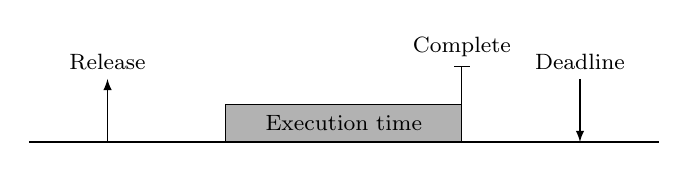
\begin{tikzpicture}[
  yscale = 0.8,
  normal/.style={fill=black!30},
  release/.style={-latex},
  complet/.style={-|},
  every text node part/.style={align=center}
]
%general params
\def\th{.6} %task height
\def\blockdim{(.4,.4)}
\def\arrowdim{(0,.5)}
\def\arrowdimB{(0,.4)}

%axes
\draw[thick, black] (0,0) -- (8, 0);

%L1
\draw[release] (1, 0) -- +(0,1) node[above] {{\footnotesize Release}};
\draw[normal]  (2.5, 0) rectangle +(3, \th) node[midway] {{\footnotesize Execution time}};
\draw[complet] (5.5, 0) -- +(0, 1.2) node[above] {{\footnotesize Complete}};
\draw[release] (7, 1) node[above] {{\footnotesize Deadline}} -- (7,0);

\end{tikzpicture}
}



\newcommand{\mrspSlideBis}{%
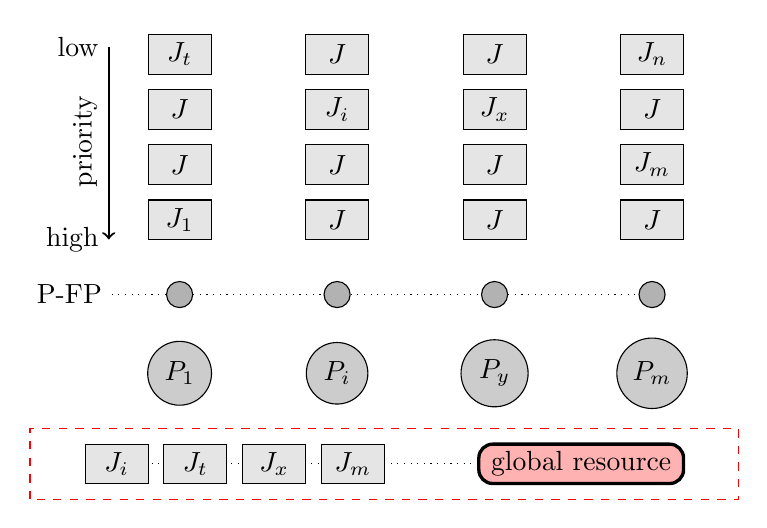
\begin{tikzpicture}[
  every text node part/.style={align=center},
  every circle node/.style={minimum width=.5ex},
  cpusty/.style={fill=gray!40,draw,circle,minimum width=1cm},
  task/.style={fill=black!10},
  sched/.style={fill=black!30,draw,circle,minimum width=1cm},
  ressty/.style={fill=red!30, draw, very thick, rounded corners=5pt}
]
%general params
\def\th{.5} %task height
\def\padding{.7}
\def\offset{.4}

% \partition{1};

  \node[cpusty] (P1) at (0+\offset,-1) {$P_1$};
  \node[sched]  (S1) at (0+\offset,0) {};

  \draw[task] (0.0,\padding*1) rectangle +(0.8, \th) node[midway,black]{$J_1$};
  \draw[task] (0.0,\padding*2) rectangle +(0.8, \th) node[midway,black]{$J$};
  \draw[task] (0.0,\padding*3) rectangle +(0.8, \th) node[midway,black]{$J$};
  \draw[task] (0.0,\padding*4) rectangle +(0.8, \th) node[midway,black]{$J_t$};

  \node[cpusty] (PI) at (2+\offset,-1) {$P_i$};
  \node[sched]  (SI) at (2+\offset,0) {};

  \draw[task] (2,\padding*1) rectangle +(0.8, \th) node[midway,black]{$J$};
  \draw[task] (2,\padding*2) rectangle +(0.8, \th) node[midway,black]{$J$};
  \draw[task] (2,\padding*3) rectangle +(0.8, \th) node[midway,black]{$J_i$};
  \draw[task] (2,\padding*4) rectangle +(0.8, \th) node[midway,black]{$J$};

  \node[cpusty] (PY) at (4.0+\offset,-1) {$P_y$};
  \node[sched]  (SY) at (4.0+\offset,0) {};

  \draw[task] (4,\padding*1) rectangle +(0.8, \th) node[midway,black]{$J$};
  \draw[task] (4,\padding*2) rectangle +(0.8, \th) node[midway,black]{$J$};
  \draw[task] (4,\padding*3) rectangle +(0.8, \th)  node[midway,black]{$J_x$};
  \draw[task] (4,\padding*4) rectangle +(0.8, \th) node[midway,black]{$J$};

  \node[cpusty] (PN) at (6.0+\offset,-1) {$P_m$};
  \node[sched]  (SN) at (6.0+\offset,0) {};

  \draw[task] (6,\padding*1) rectangle +(0.8, \th) node[midway,black]{$J$};
  \draw[task] (6,\padding*2) rectangle +(0.8, \th) node[midway,black]{$J_m$};
  \draw[task] (6,\padding*3) rectangle +(0.8, \th) node[midway,black]{$J$};
  \draw[task] (6,\padding*4) rectangle +(0.8, \th) node[midway,black]{$J_n$};
  
  \draw[dotted] (S1) -- (SI);
  \draw[dotted] (SI) -- (SY);
  \draw[dotted] (SY) -- (SN);

  \node (PFP) at (-1,0) {P-FP};
  \draw[dotted] (PFP) -- (S1);

  \draw[thick,->] (-.5,\padding*4.5) node[left,black]{low} node[rotate=90,left,xshift=-0.5cm,yshift=0.3cm]{priority} -- (-.5,\padding*1) node[left,black]{high};

  \begin{scope} [xshift=-0.8cm, yshift=-2.4cm]

  \draw[dashed, red] (-0.7,-0.2) rectangle (8.3,0.7);

  \draw[dotted] (0,0.25) -- +(5,0);
  \draw[task] (0,0) rectangle +(0.8, \th) node[midway,black]{$J_i$};
  \draw[task] (1,0) rectangle +(0.8, \th) node[midway,black]{$J_t$};
  \draw[task] (2,0) rectangle +(0.8, \th) node[midway,black]{$J_x$};
  \draw[task] (3,0) rectangle +(0.8, \th) node[midway,black]{$J_m$};

  \draw[ressty] (5,0) rectangle +(2.6,.5) node[midway]{global resource};

  % \node[inner sep=0pt] (arrow) at (8.5,1.2) {\includegraphics[width=.1\textwidth]{images/redArrow.png}};

  \end{scope}
 
\end{tikzpicture}
}

% \newcommand{\overheadsSuffered}[2]{%
% \begin{tikzpicture}[
%   xscale=#1,
%   yscale=#2,
%   every node/.append style={transform shape},
%   queuesty/.style={fill=white, very thick, font=\tiny},
%   srpsty/.style={fill=white, draw, circle, text width=.17cm, font=\tiny, very thick},
%   numsty/.style={text width=.1cm, font=\tiny},
%   arrow/.style={->},
%   littletext/.style={font=\sffamily\tiny,inner sep=0pt,outer sep=-2pt,fill=white},
%   ressty/.style={fill=red!30, draw, very thick, rounded corners=5pt},
%   emptytask/.style={rectangle, minimum width=.7cm,font=\footnotesize},
%   taskHolder/.style={fill=blue!90, draw, rectangle, minimum width=.7cm,font=\footnotesize},
%   taskWaiting/.style={fill=blue!70, draw, rectangle, minimum width=.7cm,font=\footnotesize,postaction={pattern=north east lines, very thin, pattern color=white}},
%   taskAccess/.style={fill=blue!30, draw, rectangle, minimum width=.7cm,font=\footnotesize},
%   taskNotAccess/.style={fill=white, draw, rectangle, minimum width=.7cm,font=\footnotesize}]

% \def\blockdim{(.7,.25)}

% \draw[arrow] (2.2,5.25) to[out=90,in=0] (2.35,6.6);

% \begin{scope}[xshift=2.2cm, yshift=5cm]
%   \coordinate (SRPnode) at (0,0);

%   \draw[dashed,purple] (-1.5,-0.78) -- (0.27,-0.78);

%   \node[taskNotAccess]  (T1)  at (-0.8,-0.50)  {};
%   \node[emptytask]      (TP1) at (-0.8,-0.75) {$\cdots$};
%   \node[taskWaiting]     (T2)  at (-0.8,-1.00)  {};
%   \node[emptytask]      (TP1) at (-0.8,-1.25) {$\cdots$};
%   \node[taskAccess]     (T3)  at (-0.8,-1.50)  {};
%   \node[emptytask]      (TP1) at (-0.8,-1.75) {$\cdots$};
%   \node[taskNotAccess]  (T4)  at (-0.8,-2.00)  {};
%   \node[emptytask]      (TP1) at (-0.8,-2.25) {$\cdots$};
%   \node[taskNotAccess]     (T5)  at (-0.8,-2.50)  {};

%   \draw[dashed, thin] ([shift={(-1.5,0)}]SRPnode) node[right,xshift=.1cm,littletext]{Partition$_2$} rectangle ([shift={(.3,-.15)}]T5.south-|SRPnode.east);

%   \node[srpsty] (SRP) at (SRPnode) {}; \node[font=\sffamily\tiny] at(SRPnode.west){SRP};
%   \draw[arrow] (T2.east) to[out=0,in=270] (SRP.south);

%   \draw[red] ([shift={(-.4,.17)}]T2) rectangle ([shift={(.25,-.05)}]T5.south-|T5.east);

%   \draw[arrow,red] (-0.35,-3.05) -- ([shift={(.1,-.05)}]T5.south-|T3.east);

% \end{scope}

\section{MrsP}

	\begin{frame}
	\frametitle{MrsP}
	\framesubtitle{Platform}	

		\begin{figure}
			\centering
			\scalebox{.8}{\mrspSlideBis}
			\caption{Partitioned Fixed-Priority scheduler on a platform with $m$ processors ($P_1$, \dots, $P_m$) and a global resource}
		\end{figure}

	\end{frame}

% \begin{frame}

% 	\frametitle{MrsP}
% 	\framesubtitle{Sharing resource in multiprocessor systems - 1}

% 	\begin{block}{Multiprocessor locking protocol}
% 		The serialization of access on parallel contention must guarantee:\\
% 		\begin{itemize}
% 			\item [(a)] bounded \alert{waiting time} to acquire the resource;
% 			\item [(b)] freedom from delaying repercussions for the jobs that don't require it (known as \alert{"independence preservation"}).
% 		\end{itemize}
% 	\end{block}

% 	\vspace{0.3cm}

% 	Furthermore \dots

% 	\vspace{0.3cm}

% 	\centerline{Unbounded waiting time $\rightarrow$ unbounded \alert{blocking time}}
	
% 	% An unbounded waiting time raises the \alert{blocking time} suffered by the jobs when a lower priority job will execute with an inherited ceiling priority equal or higher than its priority.\\

% \end{frame}

% \begin{frame}

% 	\frametitle{MrsP}
% 	\framesubtitle{Sharing resource in multiprocessor systems - 1}

% 	\begin{figure}
% 		\centering
% 		\scalebox{1}{\waitingtime}
% 	\end{figure}

% 	\begin{itemize}
% 		\item 2 processors and 3 tasks, $prio(J_i) > prio(J_y) \iff i > y$
% 		\item $J_1$ and $J_2$ share a global resource
% 		\item \textcolor{red}{(1)} $J_1$ remains preemptable
% 		\item \textcolor{red}{(2)} $J_1$ inhibits preemption
% 	\end{itemize}

% \end{frame}


% \begin{frame}

% 	\frametitle{MrsP}
% 	\framesubtitle{Sharing resource in multiprocessor systems - 2}

% 	\begin{block}{\emph{Suspension-based} or \emph{spin-based} protocol}
% 		A job, attempting to access a busy resource, will self-suspend ($J_2$) or will perform busy-wait ($J_3$)
% 	\end{block}

% 	\begin{figure}
% 		\centering
% 		\scalebox{0.9}{\SuspOrSpin}
% 	\end{figure}

% \end{frame}

\begin{frame}
	\frametitle{MrsP}
	\framesubtitle{Multiprocessor resource sharing Protocol - 1}

%\cite{Burns:2013:SCM:2547348.2547350}
%\cite{Baker:1991:SSR:113595.113601}

	Burns and Wellings design a multiprocessor extension of PCP/SRP with the aim of adapt a schedulability analysis to the protocol

	%in \emph{"A Schedulability Compatible Multiprocessor Resource Sharing Protocol"}

	\vspace{0.2cm}

	\begin{block}{Response Time Analysis incorporating PCP/SRP}
		The parameter \textcolor{red}{$e_j$} reflects the \textbf{contention} for the resource ($r$):

		\vspace{0.2cm}
		\centerline{$\textcolor{red}{e_j} = | map(G(r)) | \times \textcolor{blue}{c_j}$}
		\vspace{0.2cm}
		\centerline{$R_i = C_i + max \text{\{\textcolor{red}{$e_j$}},\hat{b}\} + \sum\limits_{\tau_j \in hp(i)} \ceil{\frac{R_i}{T_j}} C_j$}
		\vspace{0.2cm}
		\centerline{$C_i = WCET_i + \sum\limits_{r^j \in F(\tau_i)} n_i \text{\textcolor{red}{$e_j$}}$}

	\end{block}

\end{frame}

\begin{frame}
	\frametitle{MrsP}
	\framesubtitle{Multiprocessor resource sharing Protocol - 2}

	\centerline{\MrsP{1.1}{1.1}}

	\begingroup
 	  \fontsize{9pt}{8pt}\selectfont
	\begin{block}{Protocol's properties}
		\begin{itemize}
			\item It inherits the properties of PCP/SRP
			\item At most one job per processor requires the resource
			\item The length of the requests queue is at most $| map(G(r_j)) |$
			\item At most $e_j$ to gain the resource and to execute the critical section
		\end{itemize}
	\end{block}
	\endgroup


	% \begingroup
 	%   \fontsize{9pt}{8pt}\selectfont
	% 	\begin{enumerate}
	% 	\item access to global resources through local PCP/SRP;
	% 	\item \emph{spin at local ceiling} (remaining preemptable);
	% 	\item requests queued in a global FIFO;
	% 	\item assuming availability of a helping mechanism.
	% 	\end{enumerate}
	% \endgroup

\end{frame}

% \begin{frame}
% 	\frametitle{MrsP}
% 	\framesubtitle{Multiprocessor resource sharing Protocol - 3}	

% 	\begin{block}{Protocol's properties}
% 		\begin{itemize}
% 			\item it inherits the properties of PCP/SRP;
% 			\item at most one job per processor requires the resource;
% 			\item the length of the requests queue is at most $| map(G(r_j)) |$;
% 			\item a job requires at most $e_j$ to gain the resource and to execute the critical section.
% 		\end{itemize}
% 	\end{block}

% \end{frame}

% \begin{frame}
% 	\frametitle{MrsP}
% 	\framesubtitle{Runtime example}

% 	\centerline{\MrsPProtocols}

% 	\begin{itemize}
% 	\item $t_1$: $J_1$'s priority is raised: it gains access to $r$
% 	\item $t_2$: $J_3$'s priority is raised: it starts spinning
% 	\item $t_3$: $J_2$ is released and $J_3$ "helps" $J_1$
% 	\end{itemize}
% \end{frame}
\section{Proposed solution}

\begin{frame}

	\frametitle{Proposed solution}
	\framesubtitle{Algorithm}

	\begin{enumerate}
		\item [1)] Each resource has a set of ceilings, one for each processor
		\item [2)] An access request causes the rise of the job's priority and activates a local ceiling
		\item [3)] The requests are queued and served in arrival order
		\item [4)] A job executes, until resource's release, at the inherited priority
		\item [5)] If preempted, the lock holder migrates to the first processor available
	\end{enumerate}

	\begin{alertblock}{Key features}
		\begin{itemize}
			\item Points \textcolor{blue}{2} and \textcolor{blue}{4} make MrsP \alert{independence-preserving}
			\item Point \textcolor{blue}{5} guarantees a \alert{limited waiting and blocking time}
		\end{itemize}
	\end{alertblock}

\end{frame}
\include{04_LITMUS}
\newcommand{\partition}[1]{  


  \draw[thin]  (-0.5,-0.8) rectangle (2,3) node[right,xshift=-1cm,littletext]{Partition$_#1$};

  \draw[dashed, thin] (-0.5,2.7) node[right=0.2cm,littletext] {P-FP domain} -- +(2.5,0);

  \node[below] (F1)  at (0.8,2.50)  {\tiny (task*) scheduled};
  \node[below, xshift=-0.20cm] (F2)  at (0.8,2.20)  {\tiny (int) cpu};
  \node[below, xshift= 0.05cm] (F3)  at (0.8,1.90)  {\tiny (queue*) ready\_queue};
  \node[below, xshift=-0.45cm] (F4)  at (0.8,1.60)  {\tiny (spinlock) {lock}};
  \node[below, xshift=-0.20cm] (F5)  at (0.8,1.30)  {\tiny (sem*) mrsp};

  \draw[dashed, thin] (-0.5,0.7) node[right=0.2cm,littletext] {Local ceiling} -- +(2.5,0);

  \node[below] (F)  at (0.8,0.55)  {\tiny (int) {\color{red}ceiling}};

  \draw[dashed, thin] (-0.5,0) -- +(2.5,0);

  \node[below] (P)  at (0.75,-0.2)  {\footnotesize plugin interface};  

}


\newcommand{\mrsp}{

  \draw[thin]  (-0.5,-0.8) rectangle (2,2) node[right,xshift=-1.5cm,littletext]{Global resourse};

  \draw[dashed, thin] (-0.5,1.7) node[right=0.2cm,littletext] {MrsP} -- +(2.5,0);

  \node[below] (F1)  at (0.8,1.6)  {\tiny (task*) lock holder};
  \node[below, xshift=-0.1cm] (F2)  at (0.8,1.3)  {\tiny (int*) ceilings};
  \node[below, xshift=-0.4cm] (F3)  at (0.8,1)  {\tiny (queue*) tasks};
  \node[below, xshift=-0.5cm] (F4)  at (0.8,0.7)  {\tiny (spinlock) {lock}};

  \draw[dashed, thin] (-0.5,0.2) -- +(2.5,0);

  \node[below] (P1)  at (0.75,0.2)  {\footnotesize semaphore};
  \node[below] (P2)  at (0.75,-0.2)  {\footnotesize interface};  
}

\newcommand{\mrspRedCeiling}{

  \draw[thin]  (-0.5,-0.8) rectangle (2,2) node[right,xshift=-1.5cm,littletext]{Global resourse};

  \draw[dashed, thin] (-0.5,1.7) node[right=0.2cm,littletext] {MrsP} -- +(2.5,0);

  \node[below] (F1)  at (0.8,1.6)  {\tiny (task*) lock holder};
  \node[below, xshift=-0.1cm] (F2)  at (0.8,1.3)  {\tiny (int*) {\color{red}ceilings}};
  \node[below, xshift=-0.4cm] (F3)  at (0.8,1)  {\tiny (queue*) tasks};
  \node[below, xshift=-0.5cm] (F4)  at (0.8,0.7)  {\tiny (spinlock) {lock}};

  \draw[dashed, thin] (-0.5,0.2) -- +(2.5,0);

  \node[below] (P1)  at (0.75,0.2)  {\footnotesize semaphore};
  \node[below] (P2)  at (0.75,-0.2)  {\footnotesize interface};  
}


\newcommand{\system}[2]{
\begin{tikzpicture}[
  xscale=#1,
  yscale=#2,
  every node/.append style={transform shape},
  queuesty/.style={fill=white, very thick, font=\tiny},
  srpsty/.style={fill=white, draw, circle, text width=.17cm, font=\tiny, very thick},
  numsty/.style={text width=.1cm, font=\tiny},
  arrow/.style={->},
  littletext/.style={font=\sffamily\tiny,inner sep=0pt,outer sep=-2pt,fill=white},
  ressty/.style={fill=red!30, draw, very thick, rounded corners=5pt},
  empty/.style={rectangle, minimum width=.7cm,font=\footnotesize}]


\node[inner sep=0pt] (linux) at (0.5,2.5) {\includegraphics[width=.2\textwidth]{images/linux-logo.jpg}};

\node[inner sep=0pt] (litmus) at (3.8,2.5) {\includegraphics[width=.25\textwidth]{images/litmusrt.png}};

% /home/sebastiano/Documents/thesis/slides/images/linux-logo.jpg

\draw[fill=gray!60]  (-0.5,-0.5) rectangle (1.5,1.5)  node[midway,text width=1.9cm,align=center,font=\scriptsize] {Process management and scheduling};
\draw[fill=gray!60]  (-0.5,-2) rectangle   (1.5,-2.75)  node[midway,text width=1.9cm,align=center,font=\scriptsize] {File system};
\draw[fill=gray!60]  (-0.5,-2.75) rectangle   (1.5,-3.5)  node[midway,text width=1.9cm,align=center,font=\scriptsize] {System calls};

\draw[gray,line width=0.5mm] (2,2.5) -- (2, -3.5);

\node[inner sep=0pt] (linux) at (2,0.5) {\includegraphics[width=.09\textwidth]{images/arrow.jpg}};

\draw[fill=gray!60]  (2.5,1.2) rectangle   (5,1.95)  node[midway,text width=1.9cm,align=center,font=\scriptsize] {rt\_domain};

\draw[fill=gray!60]  (2.5,-0.8) rectangle (5,0.9) node[midway,yshift=.2cm,text width=2.1cm,align=center,font=\scriptsize] {LITMUS\textsuperscript{RT}\\scheduling class};
\draw[dashed,fill=gray!60]  (2.5,-0.3) rectangle (5,-0.8)  node[midway,align=center,font=\scriptsize] {active plugin};


\draw[fill=gray!60]  (2.5,-2) rectangle   (5,-2.75)  node[midway,text width=1.9cm,align=center,font=\scriptsize] {FDSO};
% file-descriptor-attached shared object

\draw[fill=gray!60]  (2.5,-2.75) rectangle   (5,-3.5)  node[midway,text width=1.9cm,align=center,font=\scriptsize] {System calls};

\draw[arrow] (3.75,-2.1) -- (3.75,-1.7) -- (0.25,-1.7) node[midway,yshift=0.3cm,fill=white,font=\scriptsize]{attach RT semaphores to inodes}-- (0.25,-2.1);

% \draw[fill=gray!60]  (-0.5,-2) rectangle   (1.5,-3)  node[midway,text width=1.9cm,align=center,font=\scriptsize] {System calls};

\node[empty] at (6.2,2.5) {$P_1$};
\node[empty,rotate=90] at (6.2,2) {$\cdots$}; 

\begin{scope} [xshift=7cm]
  \partition{i};
\end{scope}

\node[empty] at (9.3,2.5) {$P_m$};
\node[empty,rotate=90] at (9.3,2) {$\cdots$}; 
  
\begin{scope} [xshift=7cm,yshift=-3cm]
  \mrspRedCeiling
\end{scope}

\draw[arrow] (8.7,1) -- (9.3,1) -- (9.3,-1.3) -- (9.1,-1.3);

\def\switch{5.75}

\coordinate (D1) at (6.5,-0.4);
\draw[fill=gray] (D1) circle (.1);

\coordinate (D2) at (6.5,1.2);
\draw[fill=gray] (D2) circle (.1);

\coordinate (D3) at (6.5,-3.2);
\draw[fill=gray] (D3) circle (.1);

\coordinate (S1) at (5,-0.55);
\draw[fill=gray] (S1) circle (.1);

\coordinate (S2) at (5,1.6);
\draw[fill=gray] (S2) circle (.1);

\coordinate (S3) at (4.4,-1.37);
\draw[fill=gray] (S3) circle (.1);

\draw[arrow] ([xshift=-.1cm]D1) -- (\switch,-0.4) -- (\switch,-0.55) -- ([xshift=.1cm]S1);

\draw[arrow] ([xshift=-.1cm]D2) -- (\switch,1.2) -- (\switch,1.6) -- ([xshift=.1cm]S2);

\draw[arrow] ([xshift=-.1cm]D3) -- (\switch,-3.2) -- (\switch,-1.37) -- ([xshift=.1cm]S3);

\end{tikzpicture}}
















\newcommand{\systemOld}[2]{
\begin{tikzpicture}[
  xscale=#1,
  yscale=#2,
  every node/.append style={transform shape},
  queuesty/.style={fill=white, very thick, font=\tiny},
  srpsty/.style={fill=white, draw, circle, text width=.17cm, font=\tiny, very thick},
  numsty/.style={text width=.1cm, font=\tiny},
  arrow/.style={->},
  littletext/.style={font=\sffamily\tiny,inner sep=0pt,outer sep=-2pt,fill=white},
  ressty/.style={fill=red!30, draw, very thick, rounded corners=5pt},
  empty/.style={rectangle, minimum width=.7cm,font=\footnotesize}]

\node[empty] at (0.7,3.5) {$\cdots$}; 

\begin{scope}
  \partition{1} at (0,0);
\end{scope}

\node[empty] at (0.7,-1.5) {$\cdots$}; 

\node[empty] at (7.7,3.5) {$\cdots$}; 

\begin{scope} [xshift=7cm]
  \partition{i};
\end{scope}

\node[empty] at (7.7,-1.5) {$\cdots$}; 
  
\begin{scope} [xshift=3.5cm,yshift=0.5cm]
  \mrspRedCeiling
\end{scope}

% From sx
\draw[arrow] (1.5,1.05) to[out=0,in=180] (2.95,2);

% \draw[arrow,dashed, red, thin] (3.3,-0.4) to[out=160,in=0] (1.75,0.35);
% \draw[arrow,dashed, red, thin] (3.3,-0.45) to[out=200,in=0] (1.75,-4.2);

% From dx
\draw[arrow] (6.9,1.05) to[out=180,in=0] (5.55,2);

% \draw[arrow,dashed, red, thin] (5.1,-0.4) to[out=20,in=180] (7,0.35);
% \draw[arrow,dashed, red, thin] (5.1,-0.45) to[out=340,in=180] (7,-4.2);

\end{tikzpicture}}


\newcommand{\queueFirst}[2]{
\begin{tikzpicture}[
  xscale=#1,
  yscale=#2,
  every node/.append style={transform shape},
  queuesty/.style={fill=white, very thick, font=\tiny},
  queuestyRed/.style={fill=red!40, very thick, font=\tiny},
  queuestyGreen/.style={fill=green!50, very thick, font=\tiny},
  srpsty/.style={fill=white, draw, circle, text width=.17cm, font=\tiny, very thick},
  numsty/.style={text width=.1cm, font=\tiny},
  arrow/.style={->},
  length/.style={red, |-|, line width=1.5pt},
  littletext/.style={font=\sffamily\tiny,inner sep=0pt,outer sep=-2pt,fill=white},
  ressty/.style={fill=red!30, draw, very thick, rounded corners=5pt},
  empty/.style={rectangle, minimum width=.7cm,font=\footnotesize}]

\begin{scope}
\draw[queuestyGreen] (0,0)   rectangle +(1.4,0.8) node[midway] {\sffamily ($\tau_z$, $P_4$, {\color{red}$c_4$})};
\draw[queuestyRed] (1.4,0)   rectangle +(1.4,0.8) node[midway]{\sffamily ($\tau_j$, $P_2$, {\color{red}$c_2$})};
\draw[queuestyGreen] (2.8,0) rectangle +(1.4,0.8) node[midway]{\sffamily ($\tau_y$, $P_3$, {\color{red}$c_3$})};
\draw[queuestyGreen] (4.2,0) rectangle +(1.4,0.8) node[midway]{\sffamily ($\tau_x$, $P_1$, {\color{red}$c_1$})};
\draw[queuesty] (5.65,0) -- (5.65,0.8) -- (6,0.4) -- cycle;


\draw[length] (0,-0.6) -- (5.6,-0.6) node[left,xshift=-1cm,color=black,yshift=0.2cm]{\scriptsize FIFO length $\leq$ $| map(G(r_j)) |$ };
\end{scope}

\begin{scope} [xshift=8cm]
  \mrspRedCeiling
\end{scope}

\draw[arrow,dashed,red,thin] (7.6,0.8) to[out=180,in=0] (5.8,-0.6);

\draw[arrow,dashed,red,thin] (7.6,1.3) to[out=180,in=90] (4.9, 0.9);

\end{tikzpicture}}

\newcommand{\queueSecond}[2]{
\begin{tikzpicture}[
  xscale=#1,
  yscale=#2,
  every node/.append style={transform shape},
  queuesty/.style={fill=white, very thick, font=\tiny},
  queuestyRed/.style={fill=red!40, very thick, font=\tiny},
  queuestyGreen/.style={fill=green!50, very thick, font=\tiny},
  srpsty/.style={fill=white, draw, circle, text width=.17cm, font=\tiny, very thick},
  numsty/.style={text width=.1cm, font=\tiny},
  arrow/.style={->},
  length/.style={red, |-|, line width=1.5pt},
  littletext/.style={font=\sffamily\tiny,inner sep=0pt,outer sep=-2pt,fill=white},
  ressty/.style={fill=red!30, draw, very thick, rounded corners=5pt},
  empty/.style={rectangle, minimum width=.7cm,font=\footnotesize}]

\begin{scope}
\draw[queuestyRed] (1.4,0) rectangle +(1.4,0.8) node[midway]{\sffamily ($\tau_j$, $P_2$, {\color{red}$c_2$})};
\draw[queuestyRed] (2.8,0) rectangle +(1.4,0.8) node[midway]{\sffamily ($\tau_y$, $P_3$, {\color{red}$c_3$})};
\draw[queuestyRed] (4.2,0) rectangle +(1.4,0.8) node[midway]{\sffamily ($\tau_x$, $P_1$, {\color{red}$c_1$})};
\draw[queuesty] (5.65,0) -- (5.65,0.8) -- (6,0.4) -- cycle;

\draw[arrow,dashed,red,thin] (7.6,1.3) to[out=180,in=90] (4.9, 0.9);

\end{scope}

\begin{scope} [xshift=8cm]
  \mrspRedCeiling
\end{scope}

\end{tikzpicture}}

\newcommand{\queueThird}{
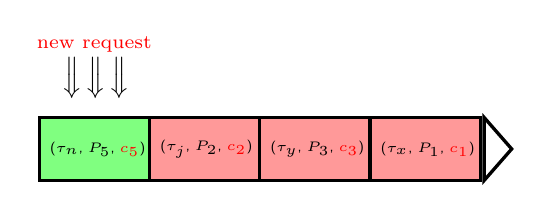
\begin{tikzpicture}[
  every node/.append style={transform shape},
  queuesty/.style={fill=white, very thick, font=\tiny},
  queuestyRed/.style={fill=red!40, very thick, font=\tiny},
  queuestyGreen/.style={fill=green!50, very thick, font=\tiny},
  srpsty/.style={fill=white, draw, circle, text width=.17cm, font=\tiny, very thick},
  numsty/.style={text width=.1cm, font=\tiny},
  arrow/.style={->},
  length/.style={red, |-|, line width=1.5pt},
  littletext/.style={font=\sffamily\tiny,inner sep=0pt,outer sep=-2pt,fill=white},
  ressty/.style={fill=red!30, draw, very thick, rounded corners=5pt},
  empty/.style={rectangle, minimum width=.7cm,font=\footnotesize}]

\begin{scope}
\draw[queuestyGreen] (0,0) node[right,yshift=0.4cm]{\sffamily ($\tau_n$, $P_5$, {\color{red}$c_5$})} rectangle +(1.4,0.8);
\draw[queuestyRed] (1.4,0) node[right,yshift=0.4cm]{\sffamily ($\tau_j$, $P_2$, {\color{red}$c_2$})} rectangle +(1.4,0.8);
\draw[queuestyRed] (2.8,0) node[right,yshift=0.4cm]{\sffamily ($\tau_y$, $P_3$, {\color{red}$c_3$})} rectangle +(1.4,0.8);
\draw[queuestyRed] (4.2,0) node[right,yshift=0.4cm]{\sffamily ($\tau_x$, $P_1$, {\color{red}$c_1$})} rectangle +(1.4,0.8);
\draw[queuesty] (5.65,0) -- (5.65,0.8) -- (6,0.4) -- cycle;

\path(0.2, 1.3)node[above,rotate=270] {${\Longrightarrow}$};
\path(0.5, 1.3)node[above,rotate=270] {${\Longrightarrow}$};
\path(0.8, 1.3)node[above,rotate=270] {${\Longrightarrow}$};
\path(0.5, 1.5)node[above,xshift=0.2cm,font=\scriptsize] {\color{red} new request};

% \draw[arrow,dashed,red,thin] (7.6,1.3) to[out=180,in=90] (4.9, 0.9);

\end{scope}

% \begin{scope} [xshift=8cm]
%   \mrspRedCeiling
% \end{scope}

\end{tikzpicture}}

\newcommand{\queueFourth}{
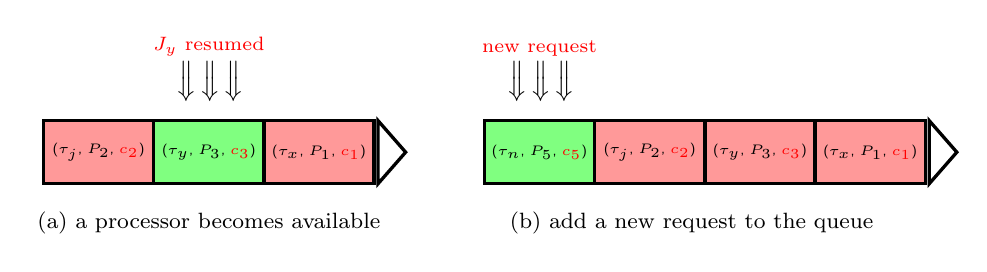
\begin{tikzpicture}[
  every node/.append style={transform shape},
  queuesty/.style={fill=white, very thick, font=\tiny},
  queuestyRed/.style={fill=red!40, very thick, font=\tiny},
  queuestyGreen/.style={fill=green!50, very thick, font=\tiny},
  srpsty/.style={fill=white, draw, circle, text width=.17cm, font=\tiny, very thick},
  numsty/.style={text width=.1cm, font=\tiny},
  arrow/.style={->},
  length/.style={red, |-|, line width=1.5pt},
  littletext/.style={font=\sffamily\tiny,inner sep=0pt,outer sep=-2pt,fill=white},
  ressty/.style={fill=red!30, draw, very thick, rounded corners=5pt},
  empty/.style={rectangle, minimum width=.7cm,font=\footnotesize}]

\begin{scope}
\draw[queuestyRed] (1.4,0)   rectangle +(1.4,0.8) node[midway]{\sffamily ($\tau_j$, $P_2$, {\color{red}$c_2$})};
\draw[queuestyGreen] (2.8,0) rectangle +(1.4,0.8) node[midway]{\sffamily ($\tau_y$, $P_3$, {\color{red}$c_3$})};
\draw[queuestyRed] (4.2,0)   rectangle +(1.4,0.8) node[midway]{\sffamily ($\tau_x$, $P_1$, {\color{red}$c_1$})};
\draw[queuesty] (5.65,0) -- (5.65,0.8) -- (6,0.4) -- cycle;

\path(3, 1.3)node[above,rotate=270] {${\Longrightarrow}$};
\path(3.3, 1.3)node[above,rotate=270] {${\Longrightarrow}$};
\path(3.6, 1.3)node[above,rotate=270] {${\Longrightarrow}$};
\path(3.3, 1.5)node[above,xshift=0.2cm,font=\scriptsize] {\color{red} $J_y$ resumed};

\path(1.2, -0.5)node[right] {{\footnotesize (a) a processor becomes available}};

% \draw[arrow,dashed,red,thin] (7.6,1.3) to[out=180,in=90] (4.9, 0.9);

\end{scope}

\begin{scope}[xshift=7cm]
\draw[queuestyGreen] (0,0) rectangle +(1.4,0.8) node[midway]{\sffamily ($\tau_n$, $P_5$, {\color{red}$c_5$})};
\draw[queuestyRed] (1.4,0) rectangle +(1.4,0.8) node[midway]{\sffamily ($\tau_j$, $P_2$, {\color{red}$c_2$})};
\draw[queuestyRed] (2.8,0) rectangle +(1.4,0.8) node[midway]{\sffamily ($\tau_y$, $P_3$, {\color{red}$c_3$})};
\draw[queuestyRed] (4.2,0) rectangle +(1.4,0.8) node[midway]{\sffamily ($\tau_x$, $P_1$, {\color{red}$c_1$})};
\draw[queuesty] (5.65,0) -- (5.65,0.8) -- (6,0.4) -- cycle;

\path(0.2, 1.3)node[above,rotate=270] {${\Longrightarrow}$};
\path(0.5, 1.3)node[above,rotate=270] {${\Longrightarrow}$};
\path(0.8, 1.3)node[above,rotate=270] {${\Longrightarrow}$};
\path(0.5, 1.5)node[above,xshift=0.2cm,font=\scriptsize] {\color{red} new request};

\path(0.2, -0.5)node[right] {{\footnotesize (b) add a new request to the queue}};

% \draw[arrow,dashed,red,thin] (7.6,1.3) to[out=180,in=90] (4.9, 0.9);

\end{scope}

% \begin{scope} [xshift=8cm]
%   \mrspRedCeiling
% \end{scope}

\end{tikzpicture}}

\section{Implementation}

% \begin{frame}

% 	\frametitle{Implementation}
% 	\framesubtitle{Development environment}

% 	The LITMUS\textsuperscript{RT} is a real-time extension of the Linux kernel.

% 	\vspace{0.3cm}
	
% 	It provides the following fundamental features:

% 	\begin{itemize}
% 		\item add a class at the top of the scheduling classes' hierarchy;
% 		\item simple plugin interface for implementing of scheduling and resource access algorithms;
% 		\item real-time domain abstraction.
% 	\end{itemize}

% \end{frame}

\begin{frame}

	\frametitle{Implementation}
	\framesubtitle{Data structures}

	\centerline{\system{1}{1}}

\end{frame}

\begin{frame}

	\frametitle{Implementation}
	\framesubtitle{Queue management - 1}

	Focused on managing the access requests queue

	\vspace{0.2cm}

	\centerline{\queueFirst{1}{1}}

	\vspace{0.2cm}

	If preempted, the lock holder ($J_x$)
		\begin{enumerate}
			\item inherits the ceiling ($c_3 + 1$)
			\item migrates to $P_3$
			\item preempts $J_y$
		\end{enumerate}
\end{frame}

\begin{frame}

	\frametitle{Implementation}
	\framesubtitle{Queue management - 2}

	% However, if there aren't available processors, the job will be re-queued in the \emph{ready\_queue}.

	The job will be re-queued in the \emph{ready\_queue}

	\vspace{0.1cm}

	\centerline{\queueSecond{1}{1}}

	\vspace{0.1cm}

	The algorithm catches the operations that 

\begin{figure}[htb]
	\centering
		\begin{subfigure}[b]{0.99\textwidth}
			\centering
			\resizebox{\linewidth}{!}\queueFourth
		\end{subfigure}
 \end{figure}
  
	% \begin{itemize}
	% 	\item add a new request to the queue
	% 	\item when a processor becomes available
	% \end{itemize}

\end{frame}

\begin{frame}

	\frametitle{Implementation}
	\framesubtitle{Primitive: mrsp\_lock}

	\begin{figure}
		\includegraphics[width=\linewidth]{../images/slides/slide_mrsp_lock.png}
	\end{figure}

\end{frame}

\begin{frame}

	\frametitle{Implementation}
	\framesubtitle{Primitive: mrsp\_unlock}

	\begin{figure}
		\includegraphics[height=7cm]{../images/slides/slide_mrsp_unlock.png}
	\end{figure}

\end{frame}

% \begin{frame}

% 	\frametitle{Implementation}
% 	\framesubtitle{Primitive: pfp\_schedule and finish\_switch}

% 	In the schedule primitive:

% 	\begin{itemize}
% 		\item a job can execute only if its priority is higher than the local ceiling;
%  		\item if preempted, the lock holder is marked for migration. 
%  	\end{itemize}

%  	After a context switch:

% 	\begin{itemize}
% 		\item the migrations take place
% 		\begin{itemize}
% 			\item the job inherites the ceiling value + 2
% 			\item it is queued in the ready\_queue;
% 		\end{itemize}
%  		\item when a waiting job resumes execution, if the lock holder has been preempted, the protocol would yield the processor to it.
%  	\end{itemize}

% \end{frame}

\begin{frame}
	\frametitle{Implementation}
	\framesubtitle{Primitive: pfp\_schedule and finish\_switch - 1}

	\centerline{\MrsPProtocolsHarder}

	\begin{itemize}
	\item $t_1$: $J_2$ is marked for migration
	\item $t_2$: $J_4$'s priority is lower than the local ceiling
	\item $t_3$: default migration mechanism
	\end{itemize}
\end{frame}

\begin{frame}
	\frametitle{Implementation}
	\framesubtitle{Primitive: pfp\_schedule and finish\_switch - 2}

	\centerline{\MrsPProtocolsHarderBis}

	\begin{itemize}
	\item $t$: $J_1$ completes and $P_1$ returns available
	\end{itemize}
\end{frame}

\newcommand{\smallqueueS}[2]{%
\draw[queuesty] (#1)node[right,xshift=.2cm,yshift=.-0.4cm]{\sffamily #2}-- ++(.2,.15)-- ++(.9,0)-- ++(0,-.3)-- ++(-.9,0)-- cycle;
\draw[fill=green!80] (#1) ++ (.3,.15)rectangle +(.3,-.3)node[font=\sffamily\tiny,inner sep=0pt,outer sep=-2pt, midway]{$L_1$};
\draw[fill=orange!80] (#1) ++ (.7,.15)rectangle +(.3,-.3)node[font=\sffamily\tiny,inner sep=0pt,outer sep=-2pt, midway]{$L_3$};}
\newcommand{\bigqueueS}[2]{%
\draw[queuesty] (#1)node[right,xshift=.2cm]{\sffamily #2}-- ++(.3,.3)-- ++(.8,0)-- ++(0,-.6)-- ++(-.8,0)-- cycle;}

\newcommand{\exampleTest}[2]{%
\begin{tikzpicture}[
  xscale=#1,
  yscale=#2,
  every node/.append style={transform shape},
  queuesty/.style={fill=white, very thick, font=\tiny},
  cpusty/.style={fill=gray!40, draw, circle, minimum width=1cm},
  srpsty/.style={fill=white, draw, circle, text width=.17cm, font=\tiny, very thick},
  numsty/.style={text width=.1cm, font=\tiny},
  ressty/.style={fill=red!30, draw, very thick, rounded corners=5pt},
  arrow/.style={->,>=stealth},
  littletext/.style={font=\sffamily\tiny,inner sep=0pt,outer sep=-2pt,fill=white},
  emptytask/.style={rectangle, minimum width=.7cm,font=\footnotesize},
  taskA/.style={fill=green!40, draw, rectangle, minimum width=.7cm,font=\footnotesize},
  taskB/.style={fill=orange!40!yellow, draw, rectangle, minimum width=.7cm,font=\footnotesize},
  task/.style={fill=white, draw, rectangle, minimum width=.7cm,font=\footnotesize}]

\begin{scope}[xshift=4cm, yshift=1cm]
\coordinate (SRP1node) at (0,0);
\node[cpusty] (P1) at (2.5,0) {$P_1$};
\node[taskA] (T1) at (1.3,0.8) {$L_1$};
\node[emptytask] (TP1) at (1.3,0.4) {$\cdots$};
\node[task] (TJ) at (1.3,0) {$J_i$};
\node[emptytask] (TP2) at (1.3,-0.4) {$\cdots$};
\node[taskA] (T2) at (1.3,-0.8) {$H_2$};
\draw[arrow] (T1.east) -- (P1.west);
\draw[arrow] (TJ.east) -- (P1.west);
\draw[arrow] (T2.east) -- (P1.west);
\draw[dashed, thin] ([shift={(-.1,.2)}]T1.north-|SRP1node) node[right,xshift=.3cm,littletext]{partition$_1$} rectangle ([shift={(.1,-.1)}]T2.south-|P1.east);
\node[srpsty] (SRP1) at (SRP1node) {}; \node[font=\sffamily\tiny] at(SRP1node.east){SRP};
\draw[arrow] (T1.west) to[out=180,in=0] ([yshift=.1cm]SRP1.east);
\node[numsty] (N1) at (0.50,.65) {}; \node[font=\sffamily\tiny] at(N1){\color{red}1};


\node[numsty] (N3) at (1.9,-.45) {}; \node[font=\sffamily\tiny] at(N3){\color{red}3};

\end{scope}

\begin{scope}[xshift=4cm, yshift=-1.1cm]
\coordinate (SRP2node) at (0,-.8);
\node[cpusty] (P2) at (2.5,-0.8) {$P_2$};

\node[task] (TX) at (1.3,0) {$J_x$};
\node[emptytask] (TP3) at (1.3,-0.4) {$\cdots$};
\node[taskB] (T3) at (1.3,-0.8) {$L_3$};
\node[emptytask] (TP4) at (1.3,-1.2) {$\cdots$};
\node[task] (TY) at (1.3,-1.6) {$J_y$};

\draw[arrow] (T3.east) -- (P2.west);
\draw[arrow] (TX.east) -- (P2.west);
\draw[arrow] (TY.east) -- (P2.west);

\draw[dashed, thin] ([shift={(-.1,.2)}]TX.north-|SRP2node) node[right,xshift=.3cm,littletext]{partition$_2$} rectangle ([shift={(.1,-.1)}]TY.south-|P2.east);
\node[srpsty] (SRP2) at (SRP2node) {}; \node[font=\sffamily\tiny] at(SRP2node.east){SRP};
\draw[arrow] (T3.west) to[out=180,in=0] (SRP2.east);
\node[numsty] (N2) at (0.6,-0.6) {}; \node[font=\sffamily\tiny] at(N2){\color{red}2};


\end{scope}

\begin{scope}
\draw[ressty] (-0.5,-.65) rectangle +(1.5,.5) node[midway, font=\tiny]{resource};
\smallqueueS{1.0,-0.4}{FIFO}
\draw[|-|] (1.2, -.02) -- ++(.9,0)node[midway,fill=white,font=\tiny]{$2$};
\end{scope}

\draw[arrow] (SRP1.west)node[anchor=south east,yshift=-.3cm,font=\tiny\sffamily]{ \begin{tabular}{c} top of access queue, \\ acquires resource \end{tabular}} to[out=180,in=0] (2.1,-.3);
\draw[arrow] (SRP2.west)node[anchor=north east,yshift=.3cm,font=\tiny\sffamily]{ \begin{tabular}{c} not top of access queue, \\ spins locally \end{tabular}} to[out=180,in=0] (2.1,-.5);

\end{tikzpicture}}

\tikzset{
%Define standard arrow tip
>=stealth',
%Define style for different line styles
help lines/.style={dashed, thick},
axis/.style={very thick, <->},
important line/.style={thick},
connection/.style={thick, dotted},
}

\newcommand{\graficoUno}{%
  \begin{tikzpicture}[
  xscale=0.7,
  yscale=0.6,
  mrsp/.style={ fill=black!30},
  pfp/.style={ fill=black!80}
  ]
    % Axis
    \coordinate (y) at (0,10);
    \coordinate (x) at (14,0);
    \draw[axis] (y) node[above=-2cm, rotate=90, font=\small] {\# Deadline miss} -- (0,0) --  (x) node[right, font=\small] {Utilization};

\draw[pfp]  (3, 8) rectangle +(1, 0.5);
\path(3.5, 8.5)node[above] {{\small P-FP}};
\draw[mrsp]  (6, 8) rectangle +(1, 0.5);
\path(6.5, 8.5)node[above] {{\small P-FP + MrsP}};

\path(2,0)node[below]{\small 50\%};
\path(4,0)node[below]{\small 60\%};
\path(6,0)node[below]{\small 70\%};
\path(8,0)node[below]{\small 75\%};
\path(10,0)node[below]{\small 80\%};
\path(12,0)node[below]{\small 85\%};

\path(2.4,.8)node[below]{\small 0};
\path(4.4,.8)node[below]{\small 0};
\path(6.4,.8)node[below]{\small 0};
\path(8.4,.8)node[below]{\small 0};

\path(1.6,.8)node[below]{\small 0};
\path(3.6,.8)node[below]{\small 0};
\path(5.6,.8)node[below]{\small 0};
\path(7.6,.8)node[below]{\small 0};

\draw[pfp]  (1.3, 0) rectangle +(0.6, 0.05);
\draw[mrsp]  (2.1, 0) rectangle +(0.6, 0.05);

\draw[pfp]  (3.3, 0) rectangle +(0.6, 0.05);
\draw[mrsp]  (4.1, 0) rectangle +(0.6, 0.05);

\draw[pfp]  (5.3, 0) rectangle +(0.6, 0.05);
\draw[mrsp]  (6.1, 0) rectangle +(0.6, 0.05);

\draw[pfp]  (7.3, 0) rectangle +(0.6, 0.05);
\draw[mrsp]  (8.1, 0) rectangle +(0.6, 0.05);

%PFP 80%
\path(9.6,1.5)node[below]{\small 102};
\draw[pfp]  (9.3, 0) rectangle +(0.6, 0.5);

% MRSP 80%
\path(10.4,1.5)node[below]{\small 102};
\draw[mrsp]  (10.1, 0) rectangle +(0.6, 0.5);

%PFP 85%
\path(11.5,9)node[below]{\small 1672};
\draw[pfp]  (11.3, 0) rectangle +(0.6, 8);

% MRSP 85%
\path(12.5,9)node[below]{\small 1672};
\draw[mrsp]  (12.1, 0) rectangle +(0.6, 8);

%50  60  70  75  80  85
%0 0 0 0 102 1672

\end{tikzpicture}}

\newcommand{\confrontoProtocolliLUno}{%
  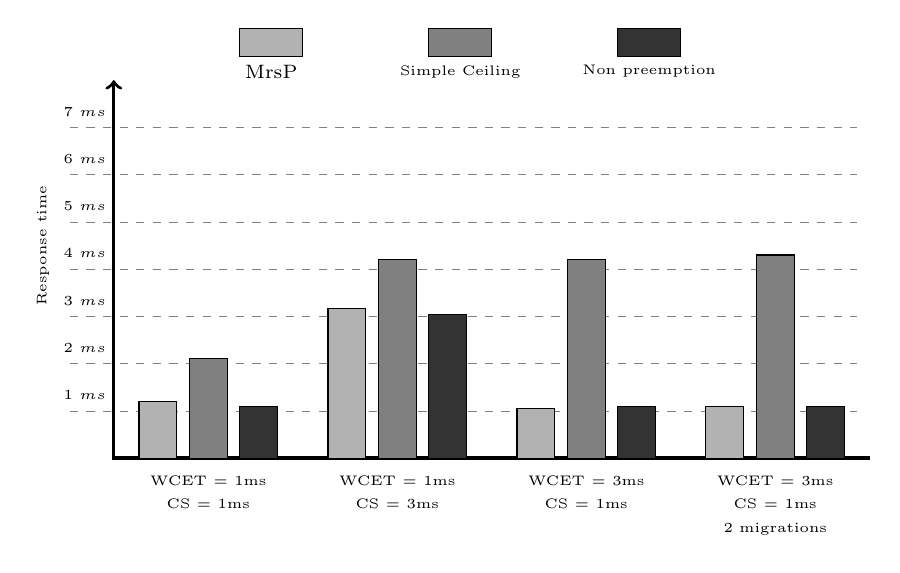
\begin{tikzpicture}[
  xscale=0.8,
  yscale=0.6,
  mrsp/.style={fill=black!30},
  ceiling/.style={ fill=black!50},
  nopreempt/.style={fill=black!80},
  assi/.style={very thick, <-}
  ]
    % Axis
    \coordinate (y) at (0,8);
    \coordinate (x) at (12,0);
    \draw[assi] (y) node[above=-3cm, right=-0.9cm, rotate=90, font=\tiny] {Response time} -- (0,0) -- (x);

    \coordinate (one) at (1.5,-0.5);
    \coordinate (two) at (4.5,-0.5);
    \coordinate (three) at (7.5,-0.5);
    \coordinate (four) at (10.5,-0.5);
%4 gruppi
%3 barre ognuno

\draw[line width=0.1mm, gray, dashed] (-0.7,1)node[black, above=0.2cm, right=-0.2cm] {\tiny 1 $ ms$} -- +(12.5, 0);
\draw[line width=0.1mm, gray, dashed] (-0.7,2)node[black, above=0.2cm, right=-0.2cm] {\tiny 2 $ ms$} -- +(12.5, 0);
\draw[line width=0.1mm, gray, dashed] (-0.7,3)node[black, above=0.2cm, right=-0.2cm] {\tiny 3 $ ms$} -- +(12.5, 0);
\draw[line width=0.1mm, gray, dashed] (-0.7,4)node[black, above=0.2cm, right=-0.2cm] {\tiny 4 $ ms$} -- +(12.5, 0);
\draw[line width=0.1mm, gray, dashed] (-0.7,5)node[black, above=0.2cm, right=-0.2cm] {\tiny 5 $ ms$} -- +(12.5, 0);
\draw[line width=0.1mm, gray, dashed] (-0.7,6)node[black, above=0.2cm, right=-0.2cm] {\tiny 6 $ ms$} -- +(12.5, 0);
\draw[line width=0.1mm, gray, dashed] (-0.7,7)node[black, above=0.2cm, right=-0.2cm] {\tiny 7 $ ms$} -- +(12.5, 0);

\path(one)node[below=+0.1cm]{\tiny CS = 1ms};
\path(one)node[below=-0.2cm]{\tiny WCET = 1ms};

\path(two)node[below=+0.1cm]{\tiny CS = 3ms};
\path(two)node[below=-0.2cm]{\tiny WCET = 1ms};

\path(three)node[below=+0.1cm]{\tiny CS = 1ms};
\path(three)node[below=-0.2cm]{\tiny WCET = 3ms};

\path(four)node[below=+0.1cm]{\tiny CS = 1ms};
\path(four)node[below=-0.2cm]{\tiny WCET = 3ms};
\path(four)node[below=+0.4cm]{\tiny 2 migrations};

%%%%%%%%%%  L1
%  MRSP - CEILING - NP

% PRIMO (1 - 1)
% $L_1$ & \underline{1.206.362} & 2.194.042 & \underline{1.111.517}

% gruppo uno - coord 0 -- 3
\draw[mrsp]  (0.4, 0) rectangle +(0.6, 1.2);
\draw[ceiling]  (1.2, 0) rectangle +(0.6, 2.1);
\draw[nopreempt]  (2, 0) rectangle +(0.6, 1.1);

% SECONDO (SC3 - h1)
%$L_1$ & \underline{3.066.828} & 4.242.092 & \underline{3.177.307}

% gruppo uno - coord 3 -- 6
\draw[mrsp]  (3.4, 0) rectangle +(0.6, 3.17);
\draw[ceiling]  (4.2, 0) rectangle +(0.6, 4.2);
\draw[nopreempt]  (5, 0) rectangle +(0.6, 3.05);

%TERZO (SC1 - H3)
%$L_1$ & \underline{1.053.232} & 4.215.599 & \underline{1.113.397}

% gruppo uno - coord 6 -- 9
\draw[mrsp]  (6.4, 0) rectangle +(0.6, 1.05);
\draw[ceiling]  (7.2, 0) rectangle +(0.6, 4.2);
\draw[nopreempt]  (8, 0) rectangle +(0.6, 1.1);

%QUARTO (SC1 - H3)^2
%$L_1$ & \underline{1.111.410} & 4.312.490 & \underline{1.173.600}

% gruppo uno - coord 9 -- 12
\draw[mrsp]  (9.4, 0) rectangle +(0.6, 1.1);
\draw[ceiling]  (10.2, 0) rectangle +(0.6, 4.3);
\draw[nopreempt]  (11, 0) rectangle +(0.6, 1.1);

%legend
\begin{scope}[shift={(2,8.5)}] 
\draw[mrsp] (0,0) rectangle +(1, 0.6) node[right=-0.4cm, below=0.35cm, color=black]{\scriptsize MrsP};
\draw[ceiling] (3,0) rectangle +(1, 0.6) node[right=-0.4cm, below=0.35cm, color=black]{\tiny Simple Ceiling};
\draw[nopreempt] (6,0) rectangle +(1, 0.6) node[right=-0.4cm, below=0.35cm, color=black]{\tiny Non preemption};
\end{scope}

\end{tikzpicture}}

\newcommand{\confrontoProtocolliHDue}{%
  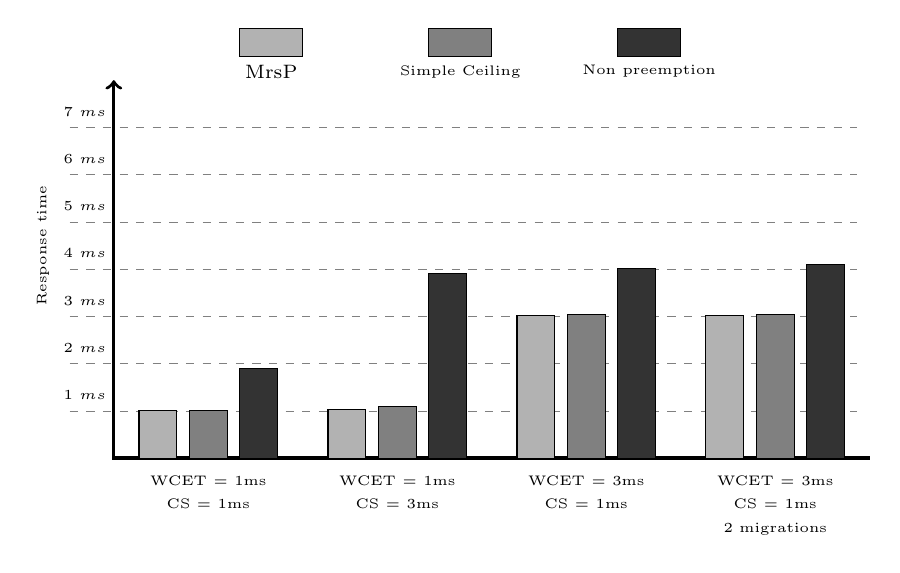
\begin{tikzpicture}[
  xscale=0.8,
  yscale=0.6,
  mrsp/.style={fill=black!30},
  ceiling/.style={ fill=black!50},
  nopreempt/.style={fill=black!80},
  assi/.style={very thick, <-}
  ]
    % Axis
    \coordinate (y) at (0,8);
    \coordinate (x) at (12,0);
    \draw[assi] (y) node[above=-3cm, right=-0.9cm, rotate=90, font=\tiny] {Response time} -- (0,0) -- (x);

    \coordinate (one) at (1.5,-0.5);
    \coordinate (two) at (4.5,-0.5);
    \coordinate (three) at (7.5,-0.5);
    \coordinate (four) at (10.5,-0.5);
%4 gruppi
%3 barre ognuno

\draw[line width=0.1mm, gray, dashed] (-0.7,1)node[black, above=0.2cm, right=-0.2cm] {\tiny 1 $ ms$} -- +(12.5, 0);
\draw[line width=0.1mm, gray, dashed] (-0.7,2)node[black, above=0.2cm, right=-0.2cm] {\tiny 2 $ ms$} -- +(12.5, 0);
\draw[line width=0.1mm, gray, dashed] (-0.7,3)node[black, above=0.2cm, right=-0.2cm] {\tiny 3 $ ms$} -- +(12.5, 0);
\draw[line width=0.1mm, gray, dashed] (-0.7,4)node[black, above=0.2cm, right=-0.2cm] {\tiny 4 $ ms$} -- +(12.5, 0);
\draw[line width=0.1mm, gray, dashed] (-0.7,5)node[black, above=0.2cm, right=-0.2cm] {\tiny 5 $ ms$} -- +(12.5, 0);
\draw[line width=0.1mm, gray, dashed] (-0.7,6)node[black, above=0.2cm, right=-0.2cm] {\tiny 6 $ ms$} -- +(12.5, 0);
\draw[line width=0.1mm, gray, dashed] (-0.7,7)node[black, above=0.2cm, right=-0.2cm] {\tiny 7 $ ms$} -- +(12.5, 0);

\path(one)node[below=+0.1cm]{\tiny CS = 1ms};
\path(one)node[below=-0.2cm]{\tiny WCET = 1ms};

\path(two)node[below=+0.1cm]{\tiny CS = 3ms};
\path(two)node[below=-0.2cm]{\tiny WCET = 1ms};

\path(three)node[below=+0.1cm]{\tiny CS = 1ms};
\path(three)node[below=-0.2cm]{\tiny WCET = 3ms};

\path(four)node[below=+0.1cm]{\tiny CS = 1ms};
\path(four)node[below=-0.2cm]{\tiny WCET = 3ms};
\path(four)node[below=+0.4cm]{\tiny 2 migrations};

%%%%%%%%%%  H2
%  MRSP - CEILING - NP

% PRIMO (1 - 1)
% $H_2$ & 1.098.587 & 1.068.602 & 1.977.039 \\

% gruppo uno - coord 0 -- 3
\draw[mrsp]  (0.4, 0) rectangle +(0.6, 1.005);
\draw[ceiling]  (1.2, 0) rectangle +(0.6, 1.008);
\draw[nopreempt]  (2, 0) rectangle +(0.6, 1.9);

% SECONDO (SC3 - h1)
%$H_2$ & 1.035.721 & 1.141.324 & 3.956.506 \\

% gruppo uno - coord 3 -- 6
\draw[mrsp]  (3.4, 0) rectangle +(0.6, 1.035);
\draw[ceiling]  (4.2, 0) rectangle +(0.6, 1.09);
\draw[nopreempt]  (5, 0) rectangle +(0.6, 3.9);

%TERZO (SC1 - H3)
%$H_2$ & 3.018.344 & 3.071.190 & 4.006.309 \\

% gruppo uno - coord 6 -- 9
\draw[mrsp]  (6.4, 0) rectangle +(0.6, 3.01);
\draw[ceiling]  (7.2, 0) rectangle +(0.6, 3.05);
\draw[nopreempt]  (8, 0) rectangle +(0.6, 4.005);

%QUARTO (SC1 - H3)^2
% $H_2$ & 3.029.214 & 3.131.630 & 4.205.578 \\

% gruppo uno - coord 9 -- 12
\draw[mrsp]  (9.4, 0) rectangle +(0.6, 3.02);
\draw[ceiling]  (10.2, 0) rectangle +(0.6, 3.05);
\draw[nopreempt]  (11, 0) rectangle +(0.6, 4.1);

%legend
\begin{scope}[shift={(2,8.5)}] 
\draw[mrsp] (0,0) rectangle +(1, 0.6) node[right=-0.4cm, below=0.35cm, color=black]{\scriptsize MrsP};
\draw[ceiling] (3,0) rectangle +(1, 0.6) node[right=-0.4cm, below=0.35cm, color=black]{\tiny Simple Ceiling};
\draw[nopreempt] (6,0) rectangle +(1, 0.6) node[right=-0.4cm, below=0.35cm, color=black]{\tiny Non preemption};
\end{scope}

\end{tikzpicture}}

\newcommand{\confrontoProtocolliLTre}{%
  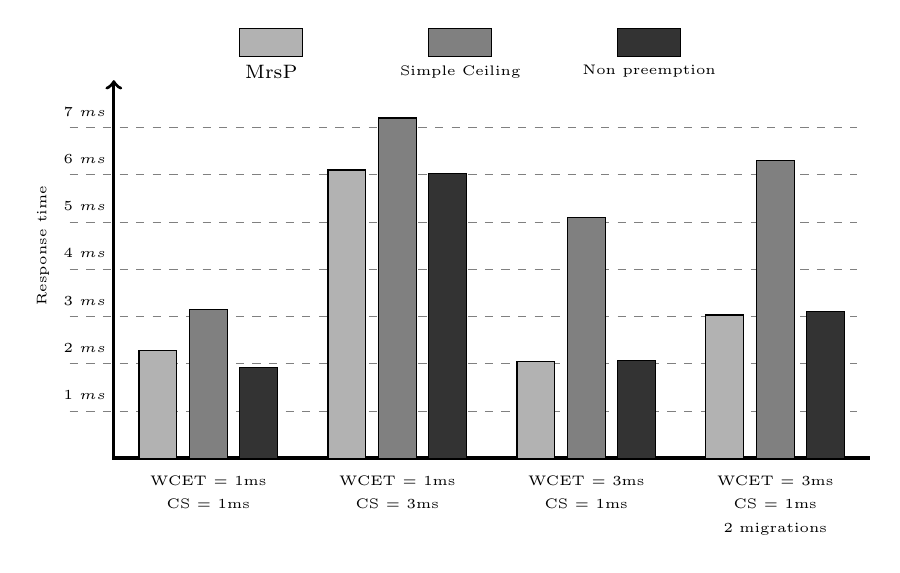
\begin{tikzpicture}[
  xscale=0.8,
  yscale=0.6,
  mrsp/.style={fill=black!30},
  ceiling/.style={ fill=black!50},
  nopreempt/.style={fill=black!80},
  assi/.style={very thick, <-}
  ]
    % Axis
    \coordinate (y) at (0,8);
    \coordinate (x) at (12,0);
    \draw[assi] (y) node[above=-3cm, right=-0.9cm, rotate=90, font=\tiny] {Response time} -- (0,0) -- (x);

    \coordinate (one) at (1.5,-0.5);
    \coordinate (two) at (4.5,-0.5);
    \coordinate (three) at (7.5,-0.5);
    \coordinate (four) at (10.5,-0.5);
%4 gruppi
%3 barre ognuno

\draw[line width=0.1mm, gray, dashed] (-0.7,1)node[black, above=0.2cm, right=-0.2cm] {\tiny 1 $ ms$} -- +(12.5, 0);
\draw[line width=0.1mm, gray, dashed] (-0.7,2)node[black, above=0.2cm, right=-0.2cm] {\tiny 2 $ ms$} -- +(12.5, 0);
\draw[line width=0.1mm, gray, dashed] (-0.7,3)node[black, above=0.2cm, right=-0.2cm] {\tiny 3 $ ms$} -- +(12.5, 0);
\draw[line width=0.1mm, gray, dashed] (-0.7,4)node[black, above=0.2cm, right=-0.2cm] {\tiny 4 $ ms$} -- +(12.5, 0);
\draw[line width=0.1mm, gray, dashed] (-0.7,5)node[black, above=0.2cm, right=-0.2cm] {\tiny 5 $ ms$} -- +(12.5, 0);
\draw[line width=0.1mm, gray, dashed] (-0.7,6)node[black, above=0.2cm, right=-0.2cm] {\tiny 6 $ ms$} -- +(12.5, 0);
\draw[line width=0.1mm, gray, dashed] (-0.7,7)node[black, above=0.2cm, right=-0.2cm] {\tiny 7 $ ms$} -- +(12.5, 0);

\path(one)node[below=+0.1cm]{\tiny CS = 1ms};
\path(one)node[below=-0.2cm]{\tiny WCET = 1ms};

\path(two)node[below=+0.1cm]{\tiny CS = 3ms};
\path(two)node[below=-0.2cm]{\tiny WCET = 1ms};

\path(three)node[below=+0.1cm]{\tiny CS = 1ms};
\path(three)node[below=-0.2cm]{\tiny WCET = 3ms};

\path(four)node[below=+0.1cm]{\tiny CS = 1ms};
\path(four)node[below=-0.2cm]{\tiny WCET = 3ms};
\path(four)node[below=+0.4cm]{\tiny 2 migrations};

%%%%%%%%%%  H2
%  MRSP - CEILING - NP

% PRIMO (1 - 1)
% $L_3$ & 2.351.562 & 3.168.240 & 1.911.890 \\

% gruppo uno - coord 0 -- 3
\draw[mrsp]  (0.4, 0) rectangle +(0.6, 2.28);
\draw[ceiling]  (1.2, 0) rectangle +(0.6, 3.15);
\draw[nopreempt]  (2, 0) rectangle +(0.6, 1.91);

% SECONDO (SC3 - h1)
%$L_3$ & 6.099.752 & 7.209.873 & 6.024.691 \\

% gruppo uno - coord 3 -- 6
\draw[mrsp]  (3.4, 0) rectangle +(0.6, 6.1);
\draw[ceiling]  (4.2, 0) rectangle +(0.6, 7.2);
\draw[nopreempt]  (5, 0) rectangle +(0.6, 6.02);

%TERZO (SC1 - H3)
%$L_3$ & 2.042.122 & 5.169.139 & 2.068.905 \\

% gruppo uno - coord 6 -- 9
\draw[mrsp]  (6.4, 0) rectangle +(0.6, 2.04);
\draw[ceiling]  (7.2, 0) rectangle +(0.6, 5.1);
\draw[nopreempt]  (8, 0) rectangle +(0.6, 2.06);

%QUARTO (SC1 - H3)^2
% $L_5$ & 3.030.634 & 6.309.370 & 3.184.333 \\

% gruppo uno - coord 9 -- 12
\draw[mrsp]  (9.4, 0) rectangle +(0.6, 3.03);
\draw[ceiling]  (10.2, 0) rectangle +(0.6, 6.3);
\draw[nopreempt]  (11, 0) rectangle +(0.6, 3.1);

%legend
\begin{scope}[shift={(2,8.5)}] 
\draw[mrsp] (0,0) rectangle +(1, 0.6) node[right=-0.4cm, below=0.35cm, color=black]{\scriptsize MrsP};
\draw[ceiling] (3,0) rectangle +(1, 0.6) node[right=-0.4cm, below=0.35cm, color=black]{\tiny Simple Ceiling};
\draw[nopreempt] (6,0) rectangle +(1, 0.6) node[right=-0.4cm, below=0.35cm, color=black]{\tiny Non preemption};
\end{scope}

\end{tikzpicture}}
\tikzset{
%Define standard arrow tip
>=stealth',
%Define style for different line styles
help lines/.style={dashed, thick},
axis/.style={very thick, <->},
important line/.style={thick},
connection/.style={thick, dotted},
}

\newcommand{\overheadsLock}{%
  \begin{tikzpicture}[
  fun/.style={ fill=black!30},
  migr/.style={ fill=black!80}
  ]
    % Axis
    \coordinate (y) at (0,9);
    \coordinate (x) at (6,0);
    \draw[axis] (y) node[above=-6cm, right=-0.9cm, rotate=90, font=\small] {Times $\mu$s} -- (0,0) --  (x);

\draw[line width=0.1mm, gray, dashed] (-0.35,1)node[black, above=0.2cm, right=-0.2cm] {\tiny 1 } -- +(6, 0);
\draw[line width=0.1mm, gray, dashed] (-0.35,2)node[black, above=0.2cm, right=-0.2cm] {\tiny 2 } -- +(6, 0);
\draw[line width=0.1mm, gray, dashed] (-0.35,3)node[black, above=0.2cm, right=-0.2cm] {\tiny 3 } -- +(6, 0);
\draw[line width=0.1mm, gray, dashed] (-0.35,4)node[black, above=0.2cm, right=-0.2cm] {\tiny 4 } -- +(6, 0);
\draw[line width=0.1mm, gray, dashed] (-0.35,5)node[black, above=0.2cm, right=-0.2cm] {\tiny 5 } -- +(6, 0);
\draw[line width=0.1mm, gray, dashed] (-0.35,6)node[black, above=0.2cm, right=-0.2cm] {\tiny 6 } -- +(6, 0);
\draw[line width=0.1mm, gray, dashed] (-0.35,7)node[black, above=0.2cm, right=-0.2cm] {\tiny 7 } -- +(6, 0);
\draw[line width=0.1mm, gray, dashed] (-0.35,8)node[black, above=0.2cm, right=-0.2cm] {\tiny 8 } -- +(6, 0);

\draw[fun]  (1, 8.5) rectangle +(0.5, 0.3);
\path(1.3, 8.9)node[above] {{\small Function}};
\draw[migr]  (3, 8.5) rectangle +(0.5, 0.3);
\path(3.3, 8.8)node[above] {{\small Migration}};

\path(1.5,0)node[below, xshift=-0.2cm]{\small PCP/SRP};
\path(3,0)node[below]{\small yield $P_i$};
\path(4.5,0)node[below]{\small busy};
\path(4.5,0)node[below, yshift=-0.3cm]{\small wait};

\draw[fun]  (1.2, 0) rectangle +(0.6, 0.8);

\draw[fun]  (2.7, 0) rectangle +(0.6, 2);
\draw[migr]  (2.7, 2) rectangle +(0.6, 6);

\draw[fun]  (4.2, 0) rectangle +(0.6, 0.5);

\end{tikzpicture}}

\newcommand{\overheadsRelease}{%
  \begin{tikzpicture}[
  fun/.style={ fill=black!30},
  migr/.style={ fill=black!80}
  ]
    % Axis
    \coordinate (y) at (0,9);
    \coordinate (x) at (4,0);
    \draw[axis] (y) node[above=-6cm, right=-0.9cm, rotate=90, font=\small] {Times $\mu$s} -- (0,0) --  (x);

\draw[line width=0.1mm, gray, dashed] (-0.35,1)node[black, above=0.2cm, right=-0.2cm] {\tiny 1 } -- +(4, 0);
\draw[line width=0.1mm, gray, dashed] (-0.35,2)node[black, above=0.2cm, right=-0.2cm] {\tiny 2 } -- +(4, 0);
\draw[line width=0.1mm, gray, dashed] (-0.35,3)node[black, above=0.2cm, right=-0.2cm] {\tiny 3 } -- +(4, 0);
\draw[line width=0.1mm, gray, dashed] (-0.35,4)node[black, above=0.2cm, right=-0.2cm] {\tiny 4 } -- +(4, 0);
\draw[line width=0.1mm, gray, dashed] (-0.35,5)node[black, above=0.2cm, right=-0.2cm] {\tiny 5 } -- +(4, 0);
\draw[line width=0.1mm, gray, dashed] (-0.35,6)node[black, above=0.2cm, right=-0.2cm] {\tiny 6 } -- +(4, 0);
\draw[line width=0.1mm, gray, dashed] (-0.35,7)node[black, above=0.2cm, right=-0.2cm] {\tiny 7 } -- +(4, 0);
\draw[line width=0.1mm, gray, dashed] (-0.35,8)node[black, above=0.2cm, right=-0.2cm] {\tiny 8 } -- +(4, 0);

\draw[fun]  (1, 8.5) rectangle +(0.5, 0.3);
\path(1.3, 8.9)node[above] {{\small Function}};
\draw[migr]  (3, 8.5) rectangle +(0.5, 0.3);
\path(3.3, 8.8)node[above] {{\small Migration}};

\path(1.5,0)node[below, xshift=-0.3cm]{\small PCP/SRP};
\path(3,0)node[below, xshift=0.3cm]{\small migrate next};
\path(3,0)node[below, yshift=-0.3cm, xshift=0.3cm]{\small lock holder};

\draw[fun]  (1.2, 0) rectangle +(0.6, 0.8);

\draw[fun]  (2.7, 0) rectangle +(0.6, 2);
\draw[migr]  (2.7, 2) rectangle +(0.6, 6);

\end{tikzpicture}}

\newcommand{\overheadsFS}{%
  \begin{tikzpicture}[
  fun/.style={ fill=black!30},
  migr/.style={ fill=black!80}
  ]
    % Axis
    \coordinate (y) at (0,9);
    \coordinate (x) at (6,0);
    \draw[axis] (y) node[above=-6cm, right=-0.9cm, rotate=90, font=\small] {Times $10 * \mu$s} -- (0,0) --  (x);

\draw[line width=0.1mm, gray, dashed] (-0.35,1)node[black, above=0.2cm, right=-0.2cm] {\tiny 1 } -- +(6, 0);
\draw[line width=0.1mm, gray, dashed] (-0.35,2)node[black, above=0.2cm, right=-0.2cm] {\tiny 2 } -- +(6, 0);
\draw[line width=0.1mm, gray, dashed] (-0.35,3)node[black, above=0.2cm, right=-0.2cm] {\tiny 3 } -- +(6, 0);
\draw[line width=0.1mm, gray, dashed] (-0.35,4)node[black, above=0.2cm, right=-0.2cm] {\tiny 4 } -- +(6, 0);
\draw[line width=0.1mm, gray, dashed] (-0.35,5)node[black, above=0.2cm, right=-0.2cm] {\tiny 5 } -- +(6, 0);
\draw[line width=0.1mm, gray, dashed] (-0.35,6)node[black, above=0.2cm, right=-0.2cm] {\tiny 6 } -- +(6, 0);

\draw[fun]  (1, 8.5) rectangle +(0.5, 0.3);
\path(1.3, 8.9)node[above] {{\small Function}};
\draw[migr]  (3, 8.5) rectangle +(0.5, 0.3);
\path(3.3, 8.8)node[above] {{\small Migration}};

\path(1.5,0)node[below, xshift=-0.2cm]{\small preempted};
\path(3,0)node[below]{\small processor};
\path(3,0)node[below,yshift=-0.3cm]{\small available};
\path(4.5,0)node[below, xshift=0.2cm]{\small default};
\path(4.5,0)node[below,yshift=-0.3cm, xshift=0.2cm]{\small migration};

\draw[fun]  (1.2, 0) rectangle +(0.6, 2.4);
\draw[migr]  (1.2, 2.4) rectangle +(0.6, 3.7);

\draw[fun]  (2.7, 0) rectangle +(0.6, 0.3);
\draw[migr]  (2.7, 0.3) rectangle +(0.6, 0.6);

\draw[fun]  (4.2, 0) rectangle +(0.6, 0.2);
\draw[migr]  (4.2, 0.2) rectangle +(0.6, 0.6);


\end{tikzpicture}}
\input{grafico_sched.tex}
\newcommand{\miss}{%
  \begin{tikzpicture}[
  xscale=0.7,
  yscale=0.6,
  mrsp/.style={ fill=black!30},
  pfp/.style={ fill=black!80},
  littletext/.style={font=\sffamily\footnotesize,inner sep=0pt,outer sep=-2pt,fill=white},
  ]
    % Axis
    \coordinate (y) at (0,10);
    \coordinate (x) at (14,0);
    \draw[axis] (y) node[above=-4.4cm, rotate=90, font=\small] {\# DL miss} -- (0,0) --  (x) node[right, font=\small] {Utilization};
    % 0.5 => 100
    % 5 => 1000
    % 7.5 => 1500

    \draw[thin, black] (-0.2, 0.5) node[left]{{\small 100}} -- (0.2, 0.5);
    \draw[thin, black] (-0.2, 5.0) node[left]{{\small 1000}} -- (0.2, 5.0);
    \draw[thin, black] (-0.2, 7.5) node[left]{{\small 1500}} -- (0.2, 7.5);



\draw[pfp]   (1.5, 8.5) rectangle +(1, 0.5) node[midway, yshift=0.4cm] {{\small P-FP}};
\draw[mrsp]  (4.5, 8.5) rectangle +(1, 0.5) node[midway, yshift=0.4cm] {{\small P-FP + MrsP}};


\node[font=\footnotesize, right] at (1,7) { Harmonic periods};
\node[font=\footnotesize, right] at (1,6.5) {WCET/period in $[0.1,0.4]$};
\node[font=\footnotesize, right] at (1,6) {Execution time: $15$ s};
\node[font=\footnotesize, right] at (1,5.5) {Processors = $4$};
\node[font=\footnotesize, right] at (1,5) {$U$ = $\{2.0, \dots , 4.0\}$};

\draw[thin] (0.8,7.7) node[right,xshift=.3cm,littletext]{Task sets} rectangle (6.7,4.5);

\path(2,0)node[below]{\small 50\%};
\path(4,0)node[below]{\small 60\%};
\path(6,0)node[below]{\small 70\%};
\path(8,0)node[below]{\small 75\%};
\path(10,0)node[below]{\small 80\%};
\path(12,0)node[below]{\small 85\%};

\path(2.4,.8)node[below]{\small 0};
\path(4.4,.8)node[below]{\small 0};
\path(6.4,.8)node[below]{\small 0};
\path(8.4,.8)node[below]{\small 0};

\path(1.6,.8)node[below]{\small 0};
\path(3.6,.8)node[below]{\small 0};
\path(5.6,.8)node[below]{\small 0};
\path(7.6,.8)node[below]{\small 0};

\draw[pfp]  (1.3, 0) rectangle +(0.6, 0.05);
\draw[mrsp]  (2.1, 0) rectangle +(0.6, 0.05);

\draw[pfp]  (3.3, 0) rectangle +(0.6, 0.05);
\draw[mrsp]  (4.1, 0) rectangle +(0.6, 0.05);

\draw[pfp]  (5.3, 0) rectangle +(0.6, 0.05);
\draw[mrsp]  (6.1, 0) rectangle +(0.6, 0.05);

\draw[pfp]  (7.3, 0) rectangle +(0.6, 0.05);
\draw[mrsp]  (8.1, 0) rectangle +(0.6, 0.05);

%PFP 80%
\draw[pfp]  (9.3, 0) rectangle +(0.6, 0.5);

% MRSP 80%
\draw[mrsp]  (10.1, 0) rectangle +(0.6, 0.5);

%PFP 85%
\draw[pfp]  (11.3, 0) rectangle +(0.6, 8);

% MRSP 85%
\draw[mrsp]  (12.1, 0) rectangle +(0.6, 8);

%50  60  70  75  80  85
%0 0 0 0 102 1672

\end{tikzpicture}}

\section{Experiments}

\begin{frame}

	\frametitle{Experiments}
	\framesubtitle{Overview}

		\begin{block}{Experiment \#1: Comparison among protocols}
			MrsP outperfmors protocols based on simple ceiling or non preemption
		\end{block}

		\begin{block}{Experiment \#2: Sampling of the overheads}
			MrsP brings benefits at reasonable costs
		\end{block}

		\begin{block}{Experiment \#3: Absence of global resources}
			The protocol doesn't interfere with the scheduler
		\end{block}

\end{frame}


\begin{frame}

	\frametitle{Experiment \#1}
	\framesubtitle{Comparison among protocols - 1}

	The experiment observes the \alert{response times} of $L_1$, $H_2$ and $L_3$ while varying the \alert{critical section length} and the \alert{WCET} of $H_2$

	\vspace{0.2cm}

    \centerline{\exampleTest{1}{1}}

\end{frame}

% \begin{frame}

% 	\frametitle{Experiments}
% 	\framesubtitle{Comparison between protocols - 2}
	
%   \begin{figure}
%     \centering
%       \begin{subfigure}[b]{0.49\textwidth}
%         \centering
%         \resizebox{\linewidth}{!}\confrontoProtocolliLUno
%         \caption{Response time of $L_1$}
%       \end{subfigure}
%       \begin{subfigure}[b]{0.49\textwidth}
%         \centering
%         \resizebox{\linewidth}{!}\confrontoProtocolliHDue
%         \caption{Response time of $H_2$}
%       \end{subfigure}
%   \end{figure}


% \end{frame}

\begin{frame}

	\frametitle{Experiment \#1}
	\framesubtitle{Comparison among protocols - 2}

	\begin{figure}
	  \centering
	  \scalebox{0.7}{\confrontoProtocolliLUno}
	  \caption{Response time of $L_1$}
	  \label{fig:test_protocols_L3}
	\end{figure}

\end{frame}

\begin{frame}

	\frametitle{Experiment \#1}
	\framesubtitle{Comparison among protocols - 3}

	\begin{figure}
	  \centering
	  \scalebox{0.7}{\confrontoProtocolliHDue}
	  \caption{Response time of $H_2$}
	  \label{fig:test_protocols_L3}
	\end{figure}

\end{frame}

\begin{frame}

	\frametitle{Experiment \#1}
	\framesubtitle{Comparison among protocols - 4}

	\begin{figure}
	  \centering
	  \scalebox{0.7}{\confrontoProtocolliLTre}
	  \caption{Response time of $L_3$}
	  \label{fig:test_protocols_L3}
	\end{figure}

\end{frame}

% \begin{frame}

% 	\frametitle{Experiments}
% 	\framesubtitle{Sampling of the overheads - 1}

% 	The experiment samples the overheads added by protocol's implementation.

% 	\begin{itemize}
% 		\item mrsp\_lock:
% 		\begin{itemize}
% 			\item [I)] local PCP/SRP
% 			\item [II)] yield the processor
% 			\item [III)] busy wait
% 		\end{itemize}
% 		\item mrsp\_unlock:
% 		\begin{itemize}
% 			\item [I)] local PCP/SRP
% 			\item [II)] migrate the next lock holder
% 		\end{itemize}
% 		\item finish\_switch:
% 		\begin{itemize}
% 			\item [I)] lock holder preempted
% 			\item [II)] processor returns available
% 			\item [III)] migration mechanism of LITMUS\textsuperscript{RT}
% 		\end{itemize}
% 	\end{itemize}

% \end{frame}

\begin{frame}

	\frametitle{Experiment \#2}
	\framesubtitle{Sampling of the overheads}

	\begin{figure}
    \centering
      \begin{subfigure}[b]{0.33\textwidth}
        \centering
        \resizebox{\linewidth}{!}\overheadsLock
        \caption{mrsp\_lock}
      \end{subfigure}
      \begin{subfigure}[b]{0.28\textwidth}
        \centering
        \resizebox{\linewidth}{!}\overheadsRelease
        \caption{mrsp\_unlock}
      \end{subfigure}
      \begin{subfigure}[b]{0.33\textwidth}
        \centering
        \resizebox{\linewidth}{!}\overheadsFS
        \caption{finish\_switch}
      \end{subfigure}
  \end{figure}

\end{frame}

\begin{frame}
	\frametitle{Experiment \#3}
	\framesubtitle{MrsP without global resources}

	The collected data show the same number of deadline miss

	\begin{figure}
    \scalebox{0.8}{\miss}
    \caption{Number of \textit{deadline miss}} %%Average job release overhead.
	\end{figure}

\end{frame}

\begin{frame}

	\frametitle{Experiment \#3}
	\framesubtitle{MrsP without global resources - pfp\_schedule performance}

	\begin{figure}[htb]
	    \centering
	      \begin{subfigure}[b]{0.49\textwidth}
	        \centering
	        \resizebox{\linewidth}{!}\graficoSchedMIN  
	        \caption{pfp\_schedule: Min}
	      \end{subfigure}
	      \begin{subfigure}[b]{0.49\textwidth}
	        \centering
	        \resizebox{\linewidth}{!}\graficoSchedMAX
	        \caption{pfp\_schedule: Max}
	      \end{subfigure}
	      \begin{subfigure}[b]{0.49\textwidth}
	        \centering
	        \resizebox{\linewidth}{!}\graficoSchedAVG
	        \caption{pfp\_schedule: Average}
	      \end{subfigure}
	  \end{figure}

  \end{frame}
% \section{Conclusion}

\begin{frame}

	\frametitle{Conclusion}
	\framesubtitle{Future work - 1}

	The experiments underline how the system suffers in case of \alert{migration}

	\vspace{0.2cm}

	\begin{block}{A possible solution}
		\begin{enumerate}
			\item Divide the resources into "long" and "short" (FMLP, \cite{Block:2007:FRL:1306877.1307316})
			\item Migration should only be caused when its benefits exceeds its cost
		\end{enumerate}	
	\end{block}

	\vspace{0.4cm}

	Supporting \alert{nested resources}

	\begin{itemize}
		\item Allow a nested request from $r_i$ to $r_j$ only if $i < j$
		\item Groups lock (FMLP)
		\item A k-lock system (RNLP, \cite{DBLP:dblp_conf/ecrts/WardA12})
	\end{itemize}

\end{frame}

\begin{frame}

	\frametitle{Conclusion}
	\framesubtitle{Future work - 2}

	Compare MrsP and the \textit{O(m) Independence-preserving Protocol}(\alert{OMIP}, \cite{6602109})
	
	\vspace{0.2cm}

	\begin{itemize}
		\item Independence preserving and limited waiting time
		\item Allows migrations
		\item Design for cluster scheduler
		\item Suspension-based
	\end{itemize}

	\begin{figure}
		\centering
		\OMIPSmall{1}{1}
	\end{figure}
	
	% With cluster size equal to one, the system is reduced to a partitioned platform.
	% MrsP and OMIP guarantee independence preserving and limited waiting time allowing migrations, but with different approaches: respectively, spin-based and suspension-based.

\end{frame}

\begin{frame}
        \frametitle{References}

        \fontsize{7pt}{7.2}\selectfont

        \bibliographystyle{plain}
		\bibliography{../reference} 
\end{frame}

% \begin{frame}
%         \frametitle{References}

%         \fontsize{7pt}{7.2}\selectfont

%         \bibliographystyle{plain}
%     \bibliography{../reference} 
% \end{frame}




% \begin{block}{Problemi aperti}
% Un numero pari $>2$ è sempre la somma di due primi?
% \end{block}
% \begin{exampleblock}{Un esempio}
% $2$ è un numero primo
% \end{exampleblock}
% \begin{alertblock}{Un errore}
% $0=1$
% \end{alertblock}












% \item generalizes uniprocessor RTA: $R_i = C_i + B_i + I_i$
%   \begin{itemize}
%     \item $I_i = \sum\limits_{\tau_j \in hp(i)} \ceil{\frac{R_i}{T_j}} C_j$
%     \item $B_i = max$\{\textcolor{red}{$\hat{c}$}$,\hat{b}\}$
%     \item $C_i = WCET_i + \sum\limits_{r^j \in F(\tau_i)} n_i \textcolor{red}{c^j}$
%   \end{itemize} 



% \begin{frame}
% \frametitle{MrsP}
% \emph{Multiprocessor resource sharing Protocol}
% \begin{itemize}
% \item for partitioned algorithms
% \item spinning-based protocol
% \item generalizes uniprocessor RTA: $R_i = C_i + B_i + I_i$
%   \begin{itemize}
%     \item $I_i = \sum\limits_{\tau_j \in hp(i)} \ceil{\frac{R_i}{T_j}} C_j$
%     \item $B_i = max$\{\textcolor{red}{$\hat{c}$}$,\hat{b}\}$
%     \item $C_i = WCET_i + \sum\limits_{r^j \in F(\tau_i)} n_i \textcolor{red}{c^j}$
%   \end{itemize} 
% \item helping mechanism
% \end{itemize}
% \end{frame}

% \begin{frame}
%   \frametitle{Overheads}

%   Resource lock:\\
%   \begin{itemize}
%     \item change priority, add job to the queue, set ceiling - 800k ns (O(m))
%     \item wake up the queued lock holder - 6k ns (migration)
%     \item busy wait - 400 ns
%   \end{itemize}

%   Resource release:
%   \begin{itemize}
%     \item restore priority, pop job from the queue, restore ceiling - 500 ns
%     \item wake up the queued lock holder - 6k ns (migration)
%     \item Running job migration - 800k ns
%   \end{itemize}

% \end{frame}

% \begin{frame}
%   \frametitle{Overheads}

%   Post context switch 1:
%   \begin{itemize}
%     \item find a new cpu for the preempted lock holder and set up the - migration 24k ns (lock cpu + lock resource)
%     \item perform the migration of the preempted job - 37k ns
%   \end{itemize}

%   Post context switch 2:
%   \begin{itemize}
%     \item a cpu is again available for a migration - 3k ns
%     \item performs the migration of the queued job - 6k ns
%   \end{itemize}  

% \end{frame}

% \begin{frame}
% \frametitle{MrsP}
% %\MrsP{1.5}{1.1}{1.1}
% \centerline{\MrsP{1}{1}}
% \end{frame}

% \begin{frame}

%   \frametitle{Response time - 1}

%   \begin{table}
%   \centering
%   \begin{tabular}{ccccc}
%   \hline\hline
%     Task & Partition     & Priority & Critical section & WCET  \\ \hline
%     $\tau_1$ & $P_1$  & 20 & 1 & 1 \\
%     $\tau_2$ & $P_2$  & 20 & 1 & 1 \\
%     \hline
%     \end{tabular}
%   \end{table}

%   \begin{table}
%   \centering
%   \begin{tabular}{cccc}
%   \hline\hline
%     Task & MrsP & Ceiling & Non preemption \\ \hline
%     $\tau_1$ & 1.123.127 & 1.045.957 & 1.181.310 \\
%     $\tau_2$ & 2.231.823 & 2.029.249 & 2.446.051 \\
%     \hline
%     \end{tabular}
%   \end{table}

% \end{frame}

% \begin{frame}

%   \frametitle{Response time - 2}

%   \begin{table}
%   \centering
%   \begin{tabular}{ccccc}
%   \hline\hline
%     Task & Partition     & Priority & Critical section & WCET  \\ \hline
%     $\tau_1$ & $P_1$  & 20 & 3 & 3 \\
%     $\tau_2$ & $P_2$  & 20 & 3 & 3 \\
%     \hline
%     \end{tabular}
%   \end{table}

%   \begin{table}
%   \centering
%   \begin{tabular}{cccc}
%   \hline\hline
%     Task & MrsP & Ceiling & Non preemption \\ \hline
%     $\tau_1$ & 3.050.809 & 3.145.418 & 3.057.504 \\
%     $\tau_2$ & 5.994.789 & 6.211.880 & 6.067.983 \\
%     \hline
%     \end{tabular}
%   \end{table}

% \end{frame}

% \begin{frame}

%   \frametitle{Response time - 3}

%   \begin{table}
%   \centering
%   \begin{tabular}{ccccc}
%   \hline\hline
%     Task & Partition     & Priority & Critical section & WCET  \\ \hline
%     $\tau_1$ & $P_1$  & 20 & 1 & 1 \\
%     $\tau_2$ & $P_1$  & 10 & 0 & 1 \\
%     $\tau_3$ & $P_2$  & 20 & 1 & 1 \\
%     \hline
%     \end{tabular}
%   \end{table}

%   \begin{table}
%   \centering
%   \begin{tabular}{cccc}
%   \hline\hline
%     Task & MrsP & Ceiling & Non preemption \\ \hline
%     $\tau_1$ & \underline{1.206.362} & 2.194.042 & \underline{1.111.517} \\
%     $\tau_2$ & 1.098.587 & 1.068.602 & 1.977.039 \\
%     $\tau_3$ & 2.351.562 & 3.168.240 & 1.911.890 \\
%     \hline
%     \end{tabular}
%   \end{table}

% \end{frame}

% \begin{frame}

%   \frametitle{Response time - 4}

%   \begin{table}
%   \centering
%   \begin{tabular}{ccccc}
%   \hline\hline
%     Task & Partition     & Priority & Critical section & WCET  \\ \hline
%     $\tau_1$ & $P_1$  & 20 & 3 & 3 \\
%     $\tau_2$ & $P_1$  & 10 & 0 & 1 \\
%     $\tau_3$ & $P_2$  & 20 & 3 & 3 \\
%     \hline
%     \end{tabular}
%   \end{table}

%   \begin{table}
%   \centering
%   \begin{tabular}{cccc}
%   \hline\hline
%     Task & MrsP & Ceiling & Non preemption \\ \hline
%     $\tau_1$ & \underline{3.066.828} & 4.242.092 & \underline{3.177.307} \\
%     $\tau_2$ & 1.035.721 & 1.141.324 & 3.956.506 \\
%     $\tau_3$ & 6.099.752 & 7.209.873 & 6.024.691 \\
%     \hline
%     \end{tabular}
%   \end{table}
% \end{frame}

% \begin{frame}
%   \frametitle{Response time - 5}

%   \begin{table}
%   \centering
%   \begin{tabular}{ccccc}
%   \hline\hline
%     Task & Partition     & Priority & Critical section & WCET  \\ \hline
%     $\tau_1$ & $P_1$  & 20 & 1 & 1 \\
%     $\tau_2$ & $P_1$  & 10 & 0 & 3 \\
%     $\tau_3$ & $P_2$  & 20 & 1 & 1 \\
%     \hline
%     \end{tabular}
%   \end{table}

%   \begin{table}
%   \centering
%   \begin{tabular}{cccc}
%   \hline\hline
%     Task & MrsP & Ceiling & Non preemption \\ \hline
%     $\tau_1$ & \underline{1.053.232} & 4.215.599 & \underline{1.113.397} \\
%     $\tau_2$ & 3.018.344 & 3.071.190 & 4.006.309 \\
%     $\tau_3$ & 2.042.122 & 5.169.139 & 2.068.905 \\
%     \hline
%     \end{tabular}
%   \end{table}

% \end{frame}

% \begin{frame}
% \frametitle{Response time - 6}
%   \begin{table}
%   \centering
%   \begin{tabular}{ccccc}
%   \hline\hline
%     Task & Partition     & Priority & Critical section & WCET  \\ \hline
%     $\tau_1$ & $P_1$  & 20 & 1 & 1 \\
%     $\tau_2$ & $P_1$  & 10 & 0 & 3 \\
%     $\tau_3$ & $P_2$  & 20 & 1 & 1 \\
%     $\tau_4$ & $P_2$  & 10 & 0 & 3 \\
%     $\tau_5$ & $P_3$  & 20 & 1 & 1 \\
%     \hline
%     \end{tabular}
%   \end{table}

%   \begin{table}
%   \centering
%   \begin{tabular}{cccc}
%   \hline\hline
%     Task & MrsP & Ceiling & Non preemption \\ \hline
%     $\tau_1$ & \underline{1.111.410} & 4.312.490 & \underline{1.173.600} \\
%     $\tau_2$ & 3.029.214 & 3.131.630 & 4.205.578 \\
%     $\tau_3$ & \underline{2.062.770} & 5.301.240 & \underline{2.211.347} \\
%     $\tau_4$ & 3.022.036 & 3.099.090 & 5.078.436 \\
%     $\tau_5$ & 3.030.634 & 6.309.370 & 3.184.333 \\
%     \hline
%     \end{tabular}
%   \end{table}

% \end{frame}

\end{document}
